%=========================================================================
% (c) Michal Bidlo, Bohuslav Křena, 2008

\iffalse

Způsoby, jak reprezentovat a uchovávat \emph{entity} existuje velké množství. V~začátcích herního průmyslu byly \emph{entity} velmi úzce provázány s~okolním kódem, ale díky velikosti týmů, které na hrách pracovaly, a relativní jednoduchosti her toto nebyl problém. Avšak s~růstem složitosti se začaly používat další přístupy, jako například \emph{objektově orientované programování}, kdy je využíván \emph{polymorfismus} a \emph{dědičnost}. 

Cílem této práce je návrh a implementace knihovny pro dynamickou kompozici objektů, za běhu aplikace. Mezi hlavní požadavky patří \emph{thread-safe}\cite{ThreadSafety} rozhraní, které je možné používat ve vícevláknových aplikacích. Další prioritou je skutečné využití a prospěch z~běhu na více vláknech, jednoduchost použití a integrace do již existujících projektů a minimalizace režie.

Práce je rozdělena do čtyř logických celků -- teoretická část\ref{Chap:Theory}, návrh systému\ref{Chap:Design}, implementace\ref{Chap:Implementation}, vyhodnocení a praktická použitelnost výsledné knihovny.

Kapitola \ref{Chap:Theory} se zabývá aktuálním stavem v~návrhu \emph{software} a důvody proč je metoda \emph{datově orientované kompozice} důležitá. Jelikož efektivní využití architektury moderních počítačů je stále více důležité, byly při návrhu knihovny použity techniky datově orientovaného návrhu\cite{DataOrientedDesign}, jehož výhody a bližší popis je součástí kapitoly \ref{Chap:DDD}. Další důležitou částí je efektivní využití vícevláknových procesorů, kterým se zabývá kapitola \ref{Chap:Parallelism}.

Kapitola \ref{Chap:Design} obsahuje obecný návrh systému pro dynamickou kompozici, který není závislý na implementačním jazyce. První část \ref{Chap:Overview} obsahuje přehled celého systému, vymezení funkcionality jednotlivých bloků a jejich komunikace. Následují sekce o~\emph{komponentech}(\ref{Chap:Component}), \emph{systémech}(\ref{Chap:System}) a \emph{entitách}(\ref{Chap:Entity}), ve kterých je specifikována jejich funkce. Návrhem paralelního přístupu a popis podporovaných možností paralelizace se zabývá sekce \ref{Chap:ParallelismDesign}.

Následuje kapitola \ref{Chap:Implementation}, ve které je popsána implementace výše zmíněného návrhu v~jazyce \emph{C++}. První část se zabývá psaním přenositelného kódu v~jazyce \emph{C++} a zdůvodnění výběru implementačního jazyka. Následuje popis implementace jednotlivých částí návrhu. Sekce \ref{Chap:CompImpl} obsahuje způsob registrace \emph{komponentů}, definuje, co může být \emph{komponentem} a základní typy datových struktur pro jejich uchovávání. Následuje popis \emph{systémů}, jejich definice a způsob, jakým jsou určeny k~používání. Dále je zde shrnuta implementace \emph{entity} a výběr mezi horizontálními a vertikálními \emph{metadaty} s~ohledem na paralelizmus. Nakonec je popsána funkce \emph{refresh} a způsoby zajištění parlelního přístupu.

Poslední část se skládá z~příkladu využití knihovny v~kapitole \ref{Chap:Demo} a vyhodnocení \ref{Chap:Eval}. Knihovna je zhodnocena z~pohledu použitelnosti (\ref{Chap:Usability}), výkonosti (\ref{Chap:Performance}) a nakonec porovnána proti vybraným \emph{open-source} knihovnám.

Jelikož se využití \emph{komponentních systémů} začalo objevovat až v~posledních letech, neexistuje obecně uznávaný způsob, jak by přesně měl vypadat. Existuje mnoho různých prací na toto téma

Právě tato metoda -- \emph{kompozice} místo \emph{dědičnosti} -- se začíná v~herním průmyslu používat stále častěji. Díky celkové neprobádanosti tohoto návrhu existuje mnoho různých způsobů jak by takový systém měl vypadat a jaké části by měl obsahovat.

Tato metoda vzniká z~použití tzv. \emph{datově orientovaného návrhu}\cite{DOD}, který se zabývá návrhem aplikací skrz analýzu a transformace dat. Jelikož je tento způsob návrhu stále vcelku nový, existuje mnoho způsobů, jak systém \emph{dynamické kompozice} navrhnout. 

Důležitou vlastností entitního systému založeného na kompozici je právě modularita, která umožňuje ...

Tato metoda vzniká z~použití tzv. \emph{datově orientovaného návrhu}\cite{DOD}.

První dokumentované použití se objevuje ve hře \emph{Dungeon Siege}\cite{DungeonSiege} \emph{Tony Hawk}, kdy \emph{Mick West} během několika let transformoval celou hierarchii na právě kompozici z~\emph{komponentů}. Následoval po

\fi

\chapter{Úvod}

Díky rostoucím požadavkům na moderní hry -- jak ve složitosti herních principů, tak i věrnosti grafické reprezentace -- se stále zvyšují požadavky na \emph{herní engine}, použitých v~jejich tvorbě. Mezi hlavní požadavky patří široké využití v~mnoha herních žánrech, možnosti multiplatformního nasazení, efektivní použití dostupného hardware, ale také jednoduchost a efektivita práce ve velkých týmech. Tyto, ale i další problémy řeší způsob návrhu pomocí \emph{Entity-component-system} paradigmatu, který v~základu používá \emph{kompozici} místo \emph{dědičnosti}.

Jelikož je tato metoda vcelku nová, širší využití začíná až v~posledních letech, existuje mnoho návrhů, jak by \emph{entitní systém} založený na kompozici měl vypadat. Nejčastěji je návrh rozdělen do tří celků -- \emph{entita}, \emph{komponent} a \emph{systém}. Výhodou je striktní oddělení logiky od dat a možnosti uložení dat do souvislých datových struktur, čímž je dosaženo efektivnější využití výpočetního hardware.

Cílem této bakalářské práce je návrh a implementace \emph{entitního systému} založeného na \emph{datově orientované kompozici}. Hlavními požadavky na tento systém jsou: 
\begin{itemize}
	\item Možnosti paralelního přístupu.
	\item Efektivní využití hardwarových prostředků.
	\item Jednoduché rozhraní a integrace do existujících projektů.
\end{itemize}
Mezi další požadavky, z~pohledu herního vývoje, jsou efektivní práce s~velkým množstvím \emph{entit}, kde většina z~nich nemusí být aktuálně používána a také komunikace mezi jednotlivými \emph{komponenty} a \emph{entitami}.

Práce je rozdělena do čtyř logických celků -- teoretická část, návrh systému, implementace a vyhodnocení. Kapitola teorie (\ref{Chap:Theory}) popisuje aktuální stav návrhu software, z~pohledu vývoje her a důvody vzniku \emph{ECS} paradigmatu. Nejdříve jsou zde přiblíženy požadavky na \emph{entitní systémy}, následuje porovnání aktuálně používaných způsobů reprezentace \emph{entit} a srovnání jejich výhod a nevýhod. Závěr se zabývá způsoby, jak využít více-jádrové hardwarové konfigurace. Kapitola návrh (\ref{Chap:Design}) zahrnuje kompletní návrh \emph{entitního systému}, který je obecný -- nezávislý na implementačním jazyce. Úvod obsahuje přehled celého systému, další sekce pokračují podrobnějším popisem jeho částí a rozborem různých způsobů řešení. Následující kapitola -- implementace (\ref{Chap:Implementation}) -- je věnována implementaci výše zmíněného návrhu v~programovacím jazyce \emph{C++}. Závěrečná kapitola (\ref{Chap:Results}) shrnuje vlastnosti výsledného systému z~pohledu výkonosti a srovnává jej s~podobnými volně dostupnými knihovnami.

\chapter{Teoretický rozbor}
\label{Chap:Theory}

Tato kapitola se věnuje teorii \emph{entitních systémů}, jejich historii a požadavkům na ně kladeným. Dále obsahuje rozbor běžně používaných způsobů reprezentace \emph{entit} a srovnává jejich výhody a nevýhody. Následuje popis vlastního \emph{entitního systému} založeného na \emph{ECS} paradigmatu a definice hlavních pojmů -- \emph{entita}, \emph{komponent} a \emph{systém}. Na závěr se věnuje metodám paralelizmu, které budou zváženy pro následující návrh entitního systému.

\section{Entitní systémy}

\emph{Entitní systém} je část herního enginu, který zprostředkovává správu \emph{entit} -- objektů ve virtuálním světě. Alternativní název pro \emph{entitu}, který se také často používá, je \emph{herní objekt} (\emph{Game Object} \cite{UnityGo}). Primární funkcí \emph{entit} je propojení jednotlivých modulů a částí aplikace, které jsou vyvíjeny odděleně -- např. herní logika a simulace fyziky.

\section{Požadavky na návrh}

Stále zvyšující se požadavky na složitost herních principů, věrnost grafické reprezentace a velikost virtuálních světů mnohonásobně ztěžují návrh \emph{herních enginů}, na kterých jsou hry stavěny. Dalším problémem je znovupoužitelnost již vytvořených částí, nejen ve stejném projektu, ale stále častěji i v~dalších hrách. Z~výše zmíněných důvodů vznikají techniky pro organizaci kódu a knihy \emph{návrhových vzorů} \cite{DesignPatterns, GameDesignPatterns}, které obsahují zkušenosti a prověřené způsoby jak navrhovat software. Důležitou vlastností správného návrhu, je také modularita -- oddělení částí systému -- která umožňuje velkému množství programátorů pracovat na jednom projektu. Základem \emph{Entity-Component-System} paradigmatu je striktní oddělení logiky a dat, čímž je umožněna vysoká úroveň modularity. 

Způsob reprezentace \emph{entit} -- objektů ve virtuálním světě -- je jedním z~důležitých rozhodnutí v~návrhu \emph{herního enginu}. Entity jsou často používány pro komunikaci mezi jednotlivými podsystémy -- např. přidání efektu z~herní logiky. Přílišná provázanost však většinou znamená zvýšený výskyt programovacích chyb (\emph{bugs}) \cite{GameDesignPatterns}. Podrobněji se tímto zabývá sekce \ref{Chap:Representation}.

\section{Architektura moderních počítačů}

Důležitou součástí tvorby her je analýza cílové platformy, na které hra poběží. Velkou výhodou je v~dnešní době podobnost všech různých herních systémů. Stolní počítače, ale i některé nové herní konzole (\emph{Playstation 4} a \emph{Xbox One} \cite{Ps4Xbox}), používají architekturu procesorů \emph{x86} \cite{IntelX86-64, AmdX86-64}. Stále důležitější platformou jsou také mobilní zařízení, které většinou používají architekturu procesorů \emph{ARM} \cite{ARM}. Díky podobnosti paměťových hierarchií na těchto platformách, je možné implementovat optimalizace, které vylepšují výkon výsledných aplikací na všech cílových systémech.

Moderní procesory dokáží velmi rychle vykonávat jednoduché instrukce a za použití mechanizmů (např. \emph{pipelining} \cite{Pipelining}) se stále zvyšuje počet instrukcí za jeden cyklus (\emph{Instructions per Cycle} \cite{CpuIpc}). Problém nastává v~případě, kdy procesor operuje s~daty, které nejsou k~dispozici v~jeho registrech, jelikož rozdíl v~rychlosti procesorů a pamětí stále roste \cite{CpuMemoryGap}. Kvůli těmto rozdílům existuje hierarchie procesorových vyrovnávacích pamětí (\emph{cache}), jejichž cílem je minimalizace rozdílů rychlostí jednotlivých pamětí.

Právě díky rozdílům rychlostí jednotlivých typů pamětí \cite{MemoryTiming} vznikají nové způsoby, jak navrhovat aplikace, které umožňují efektivně využívat hierarchii procesorových vyrovnávacích pamětí. Jedním z~nich je \emph{datově orientovaný} návrh, ze kterého vychází \emph{ECS} paradigma.

Mezi důležité parametry pro efektivní využití \emph{cache} patří lokalita dat \cite{DataLocality} a -- v~případě více-jádrových systému -- udržování jejich koherence \cite{CacheCoherence}. Lokalita dat je primárně dělena na 2 typy -- časová a prostorová. Časovou lokalitou je myšleno opakované používání stejných dat, kdy se při prvním použití data přesunou do vyrovnávací paměti  a dále je k~nim již přistupováno skrz rychlejší paměť. Načítání dat do \emph{cache} je prováděno v~blocích (\emph{cache line}), jejichž velikost je specifická pro každý procesor. Program, který přistupuje k~datům, jejichž vzdálenost v~paměti není příliš velká (vejdou se do jedné \emph{cache line}) využívá prostorové lokality dat, kdy výsledkem je méně přístupů do pomalejších pamětí. Udržování koherence procesorových \emph{cache} se primárně projevuje ve více-jádrových systémech a podrobněji se jím zabývá sekce \ref{Chap:Parallelism}.

\section{Datově orientovaný návrh}
\label{Chap:DDD}

Dnes nejpoužívanější způsob návrhu -- \emph{objektově orientovaný} (\emph{OOD}) -- umožňuje abstrahovat od fyzického hardware, na kterém výsledná aplikace běží a řešit daný problém jeho dekompozicí do tříd. Základní stavební jednotkou je v~tomto případě třída -- agregace hodnot a  množiny operací nad ní proveditelnou. Toto umožňuje řešení problémů transformací objektů z~reálného světa na objekty virtuální, se kterými dokáží lidé pracovat a zároveň jsou interpretovatelné i překladači programovacích jazyků. Toto je však problematické pro moderní výpočetní hardware, který je velmi výkonný v~případě opakovaného provádění jednoduchých datových transformací. Dalším problémem je využití pouze části dat, která daný objekt obsahuje, čímž jsou tato data zbytečně načtena do vyrovnávací paměti.

Kvůli výše zmíněným problémům vzniká \emph{datově orientovaný návrh}\cite{DOD} (\emph{DOD}), jehož cílem, na rozdíl od \emph{OOD}, je analýza dat, se kterými aplikace pracuje a následovné použití jednoduchých transformací. Nevýhodou využití \emph{OOD} je snížení čitelnosti výsledného kódu a složitější transformace návrhu aplikace -- řešení problému -- ve výsledný program. Základní myšlenkou je oddělení dat a operací nad nimi, čímž je umožněno efektivnějšího využití procesorových vyrovnávacích pamětí.

Základem \emph{DOD} je důkladná analýza aplikačních dat -- jejich obor hodnot, transformace, definice vstupních dat, požadovaný výstup atp. Často je využíváno datové struktury pole, jejíž vlastnosti umožňují rychlou iteraci. Mezi výhody \emph{DOD} patří také lepší lokalita dat, čímž je zvýšena datová propustnost výsledné aplikace. Díky těmto vlastnostem je \emph{DOD} často využíván při návrhu software, který vyžaduje vysokou úroveň optimalizace -- v~tomto případě při návrhu her\cite{DataOrientedDesignDice, DataOrientedDesignCppCon}.

Častým příkladem rozdílů mezi \emph{OOD} a \emph{DOD} je transformace pole struktur (\emph{AOS}) v~strukturu polí (\emph{SOA}), jejíž ilustraci lze vidět na obr. \ref{Fig:SOAASO}.

\begin{figure}[]
	\centering
	\tmpframe{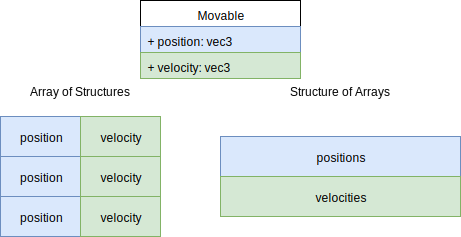
\includegraphics[width=0.6\linewidth]{BAC-DOD1}}
	\caption{Příklad transformace pole struktur na strukturu polí.}
	\label{Fig:SOAASO}
\end{figure}

%Entitní systém navržený v této práci vychází z principů \emph{DOD} -- \emph{datově orientovaná kompozice}\cite{DODComponents}. Blíže se tímto způsobem skládání \emph{entit} zabývá sekce \ref{Chap:DOC}.

\section{Reprezentace entit}
\label{Chap:Representation}

Tato sekce obsahuje rozbor nejpoužívanějších způsobů reprezentace \emph{entit} \cite{EvolveHierarchy} a jejich \emph{chování}. Pod pojmem \emph{entita} je myšlen objekt ve virtuálním světě. \emph{Chování}, nebo \emph{aspekt}, definuje operace, které \emph{entita} dokáže provést -- pohyb, vykreslení, kolize atp.

Pro ilustraci návrhu pomocí jednotlivých metod je použit ukázkový návrh jednoduché 2D \uv{shoot'em up} hry, kde prezentovaný návrh není nutně optimální, ale ukazuje vlastnosti dané metody. Dílčí reprezentace entit jsou hodnoceny na základě složitosti implementace, návrhu s~jejich použitím a výhodnosti z~pohledu hardware. Závěry zde vyvozené jsou primárně zaměřené na \emph{třídní} objektově orientované jazyky (\emph{C++}, \emph{JAVA}, \emph{Python} atp.), ale částečně je lze aplikovat i na \emph{objektově orientované} programovací jazyky obecně.

\subsection{Objektově orientovaná hierarchie}

Pod pojmem \emph{objektově orientovaná hierarchie} (\emph{OOH} \cite{GameDesignPatterns}) je míněn způsob skládání nových typů entit za využití \emph{dědičnosti}. Příklad hierarchie, navržené pro ukázkovou 2D hru, lze vidět na obr. \ref{Fig:OOPHierarchy}. V~kořenu stromu hierarchie je, v~případě \emph{OOH}, bázová třída, která umožňuje uniformní skladování entit. Konkrétní entity, které existují v~herním světě, jsou listy ve stromu dědičnosti.

Množina akcí entity je nastřádána průchodem stromu dědičnosti od kořene k~listu, kde se konkrétní entita nachází. Existují dva často používané způsoby definice těchto akcí, kdy u~první z~nich je akce specifikována přímo v~supertřídě. Druhým je potom použití \emph{polymorfizmu}, kdy děděné třídy specifikují pouze, že akce by měla existovat, ale definici nechávají na podtřídě.

\begin{figure}[H]
	\tmpframe{\includegraphics[width=\linewidth]{BAC-OOP1}}
	\caption{Příklad objektově orientované hierarchie.}
	\label{Fig:OOPHierarchy}
\end{figure}

Hierarchii dědičnosti, která je v~tomto příkladě použita lze vidět na obr. \ref{Fig:OOPHierarchy}. Bázová třída \textbf{Entity} obsahuje kód pro vykreslování, dále se hierarchie dělí na \emph{entity} pohyblivé a statické. Prvním problémem je umístění entit, které jsou v~pozadí -- nelze do nich narazit. V~tomto případě je nutné rozdělit nepohyblivé \emph{entity} do dvou podtypů, čímž dochází k~duplikaci kódu ve třídách \textbf{Meteorite} a \textbf{BgMeteorite}. Dalším příkladem problémů s~\emph{OOH} je přidání nepohyblivá zbraně -- třídy \textbf{StationaryGun}. Zbraň je v~tomto případě nepřítelem, ale zároveň je také nepohyblivá. Tyto problémy lze u~prezentované hierarchie opravit, ale pro větší projekty to již nemusí být možné. 

\begin{figure}[H]
	\centering
	\tmpframe{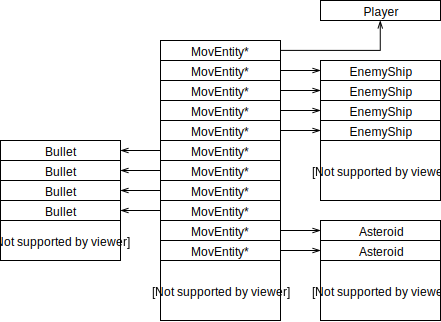
\includegraphics[width=0.6\linewidth]{BAC-OOP2}}
	\caption{Příklad obsahu paměti, při využití \emph{objektově orientované hierarchie}.}
	\label{Fig:OOPMemory}
\end{figure}

Pro příklad využití paměti je využit seznam pohybujících se entit, jejichž pozice musí být každý snímek hry aktualizována, aplikací jejich rychlosti. Ilustraci možné organizace paměti lze vidět na obr. \ref{Fig:OOPMemory}. Středem je pole ukazatelů, které obsahuje entity, které je potřeba aktualizovat. Instance jednotlivých konkrétních typů jsou uloženy v~oddělených polích.

\begin{figure}[H]
	\centering
	\tmpframe{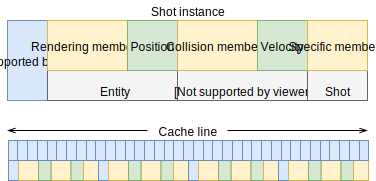
\includegraphics[width=0.6\linewidth]{BAC-OOP3}}
	\caption{Využití vyrovnávací paměti při použití \emph{objektově orientované} entitní hierarchie. Uvedený příklad pracuje s~objektem \uv{střely}.}
	\label{Fig:OOPCache}
\end{figure}

Při operaci aktualizace je iterováno přes hlavní pole ukazatelů a na každý objekt je aplikována metoda, která aktualizuje jeho pozici přičtením rychlosti. Postup práce s~hlavní pamětí a hierarchií vyrovnávacích pamětí je následující\footnote{Postup neuvažuje různé vrstvy paměti \emph{cache} a předpokládá, že k~požadovanému bloku paměti zatím nebylo přistoupeno. Velikost řádku vyrovnávací paměti je nastavena tak, aby nedošlo k~překrytí paměti ukazatelů a paměti instancí.}. Prvním krokem je načtení bloku paměti, který obsahuje část pole ukazatelů do vyrovnávací paměti. Následuje dereference prvního z~ukazatelů, která zapříčiní přesun dalšího řádku paměti, který již obsahuje iterované objekty. Ilustrace obsahu paměti \emph{cache} lze vidět na obr. \ref{Fig:OOPCache}. Entity kromě požadovaných informací -- pozice a rychlost -- obsahují také data, která nejsou využita. Výsledkem je neoptimální využití procesorových \emph{cache} \cite{DataOrientedDesignDice}.

Komunikace jednotlivých částí je při použití \emph{OOH} implicitní -- pomocí \emph{public} a \emph{protected} členů. 

\noindent Mezi výhody \emph{OOH} patří: 
\begin{itemize}
	\item Podpora tříd zabudována do mnoha programovacích jazyků.
	\item Použití standardních návrhových metod z~objektově orientovaného návrhu.
	\item Implicitní propojení a komunikace mezi děděnými částmi.
\end{itemize}

\noindent Její nevýhody jsou: 
\begin{itemize}
	\item Akumulace stavu a chování, které není nutně entitou vyžadováno.
	\item Duplikace kódu v~různých větvích stromu dědičnosti.
	\item Zvyšující se složitost umisťování nových typů entit.
	\item Typy entit jsou specifikovány ve zdrojovém kódu.
	\item Statické typování\footnote{Může být výhodou v~některých případech, např. optimalizace, které vykonává překladač.}, nemožnost tvorby nových typů za běhu programu.
\end{itemize}

\subsection{Objektově orientovaná kompozice}

Pod pojmem \emph{objektově orientovaná kompozice} (\emph{OOC} \cite{GameDesignPatterns}) je myšlena tvorba entit z~menších částí -- komponent -- kde komponenty obsahují data a množinu proveditelných akcí. Entita je při použití \emph{OOC} kontejner, který obaluje seznam komponent (\emph{kompozice}). Příklad návrhu množiny komponent lze vidět na obr. \ref{Fig:OOCHierarchy}, kontejnerem je v~tomto případě třída \textbf{Entity}.

\begin{figure}[H]
	\centering
	\tmpframe{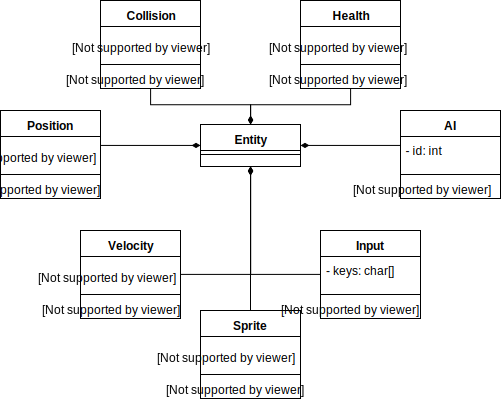
\includegraphics[width=0.7\linewidth]{BAC-OOC1_1}}
	\caption{Příklad objektově orientované kompozice.}
	\label{Fig:OOCHierarchy}
\end{figure}

Jelikož komponenty obsahují kromě dat také akce, lze množinu akcí, kterou lze nad výslednou entitou provést, definovat jako sjednocení množin akcí jednotlivých vlastněných komponent. Tato vlastnost umožňuje dynamickou tvorbu entit za běhu aplikace, jejichž chování je definováno přítomnými komponentami.

Tato metoda je často používána\footnote{\uv{Composition over inheritance}} v~návrhu software a je mezikrokem od \emph{objektově orientované hierarchie} k~\emph{datově orientované kompozici}. 

Příkladem využití těchto komponent, pro implementaci stejné množiny konkrétních entit, jako v~případě použití \emph{OOH}, lze vidět na obr. \ref{Fig:OOCEntity}. Oproti využití dědičnosti se zde již lze jednoduše vyhnout problému s~umístěním entit do stromu dědičnosti. Přidání typu \textbf{StationaryGun} je již také bezproblémové, díky možnosti libovolné kombinace jednotlivých komponent.

\begin{figure}[H]
	\centering
	\tmpframe{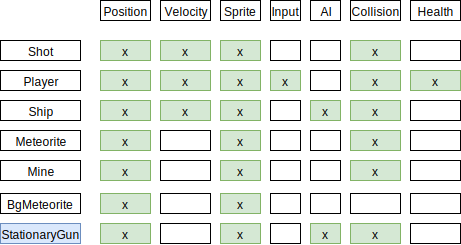
\includegraphics[width=0.7\linewidth]{BAC-OOC1_2}}
	\caption{Využití kompozice pro tvorbu herních objektů. Konkrétní typy entit jsou zde reprezentovány řádky, jednotlivé komponenty jsou potom sloupce. Přítomnost komponenty je vyznačena znakem \uv{\emph{x}}.}
	\label{Fig:OOCEntity}
\end{figure}

Existuje mnoho způsobů, jak tuto základní myšlenku kompozice z~menších částí implementovat. Jednou z~možností je vyhradit pro každý typ komponenty pozici v~seznamu ukazatelů\footnote{Mezi další způsoby patří mapy nebo dynamické seznamy. Možným řešením je také použití obecných ukazatelů a typových proměnných. }. V~tomto návrhu je entita redukována na seznam ukazatelů, kde každá komponenta je buď přítomna (ukazatel je nastavený), nebo nepřítomna (ukazatel je \emph{NULL}). Výhodou této implementace je rychlost, nevýhodou je využití paměti, pro větší množství druhů komponent. Ilustraci této implementace lze vidět na obr. \ref{Fig:OOCImpl}. 

\begin{figure}[H]
	\centering
	\tmpframe{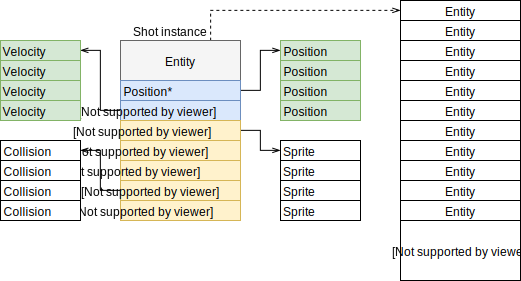
\includegraphics[width=0.7\linewidth]{BAC-OOC2}}
	\caption{Obsah paměti u~\emph{objektově orientované kompozice}. Zde je entita implementována pomocí seznamu ukazatelů.}
	\label{Fig:OOCImpl}
\end{figure}

Jako příklad práce s~pamětí je opět použita iterace nad seznamem entit, u~kterých je nutno provést aktualizaci pozice přičtením jejich rychlosti. V~tomto příkladě je použita implementace pomocí statického seznamu ukazatelů, podle obr. \ref{Fig:OOCImpl}.

Podobně, jako při použití \emph{OOH}, je zde iterováno nad polem entit, který však tentokrát obsahuje již jednotlivé instance typu \textbf{Entity}\footnote{Předpokládá se, že všechny entity obsahují komponenty typu \textbf{Position} a \textbf{Velocity}.}. Využití vyrovnávací paměti, za stejných předpokladů, jako v~případě \emph{OOH}, je následující. Nejdříve je načten seznam entit a jejich ukazatelů na jednotlivé komponenty. Požadovaná operace potřebuje pouze ukazatele na komponenty typu \textbf{Position} a \textbf{Velocity}, ostatní jsou v~tomto případě zbytečné. Následuje přístup k~požadovaným komponentám skrz ukazatele v~první entitě. Tímto je načten blok paměti, pro každou komponentu, do vyrovnávací paměti. Po provedení první operace jsou již následující komponenty přístupné z~vyrovnávací paměti. 

\begin{figure}[H]
	\centering
	\tmpframe{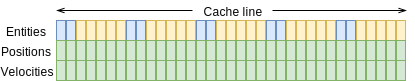
\includegraphics[width=0.7\linewidth]{BAC-OOC3}}
	\caption{Využití procesorové \emph{cache} při použití objektově orientované kompozice.}
	\label{Fig:OOCCache}
\end{figure}

Komunikace mezi jednotlivými komponenty je při použití \emph{objektově orientované kompozice} problematické. Jelikož jsou jednotlivé komponenty samostatné objekty, nepřístupné z~ostatních komponent stejné entity, není mezi nimi možná přímá komunikace. Jedním možným řešením je přidání systému zpráv, který má přístup k~celé entitě, včetně jejích komponent. Dílčí komponenty se následně mohou dotazovat na typy zpráv, které je zajímají, nebo je možné využít návrhového vzoru \emph{pozorovatel}. Dalším řešením je umožnit komponentám přímou komunikace předáním ukazatelů na entitu, nebo na další komponentu, se kterou může daná komponenta komunikovat. Nevýhodou v~případě přímé komunikace je bližší vazba výsledných komponent, což může způsobit chyby při změně některé z~komunikujících stran.

\noindent Mezi výhody \emph{OOC} patří: 
\begin{itemize}
	\item Uniformní instance všech typů entit, liší se pouze v~přítomných komponentách.
	\item Lepší využití vyrovnávacích pamětí.
	\item Možnost definování nových typů entit za běhu, použitím kompozice.
	\item Komponenty, které entita vlastní, jsou přístupny z~jednoho místa.
	\item Odstraněna duplikace kódu a akumulace nechtěného stavu.
\end{itemize}

\noindent Její nevýhody jsou: 
\begin{itemize}
	\item Složitější implementace, většinou bez podpory v~programovacím jazyce.
	\item Komunikace mezi komponentami není implicitní, je nutno ji implementovat. 
\end{itemize}

\pagebreak

\subsection{Datově orientovaná kompozice}
\label{Chap:DOC}

\emph{Datově orientovaná kompozice} (\emph{DOC}) je dalším krokem v~separaci dat a logiky. Podobně, jako \emph{objektově orientovaná kompozice}, \emph{DOC} rozděluje entity do menších části -- komponent -- což umožňuje vyšší modularitu výsledného návrhu. Oproti \emph{OOC} však dochází ke kompletní separaci logiky a~dat, kdy komponenty již neobsahují kód akcí\footnote{Logikou je v~tomto případě myšleno kód, který pracuje na vyšší úrovni, než pouze s~daty dané komponenty. Blíže k~tomuto tématu v~sekci \ref{Chap:EntitySystem}}.

Množinu akcí, které lze nad entitou vykonat, je opět definována přítomnými komponentami. Jelikož komponenty samy o~sobě neobsahují logiku, je nutno akce definovat v~okolním kódu. Jedním způsobem je přímý přístup ke komponentám a jejich datům, tato metoda bude použita v~následujícím příkladě. Pro rozsáhlejší aplikace, kde je potřeba lepší kontrola nad přístupy k~jednotlivým komponentám, lze například využít \emph{systémy}, které implementují akce nad komponenty\footnote{Tato metoda je blíže popsána v~sekci \ref{Chap:EntitySystem}}. Tento způsob je využit i v~návrhu \emph{entitního systému}, o~kterém je napsána tato práce.

\begin{figure}[H]
	\centering
	\tmpframe{\includegraphics[width=0.7\linewidth]{BAC-DOC1_1}}
	\caption{Příklad datově orientované kompozice a návrh komponent, které tvoří výsledné entity.}
	\label{Fig:DOCHierarchy}
\end{figure}

Příklad návrhu entity a komponent lze vidět na obr. \ref{Fig:DOCHierarchy}. Mezi důležité změny, oproti \emph{OOC}, patří veřejný (\emph{public}) přístup k~atributům komponent. Entita je v~tomto návrhu reprezentována číslem -- \emph{identifikátorem} -- skrz který lze komponenty jednoznačně přiřadit k~entitám, které je vlastní. Implementace konkrétních entit je konceptuálně stejná, jako při použití \emph{objektově orientované kompozice}, příklad lze vidět na obr. \ref{Fig:OOCEntity}.

\begin{figure}[H]
	\centering
	\tmpframe{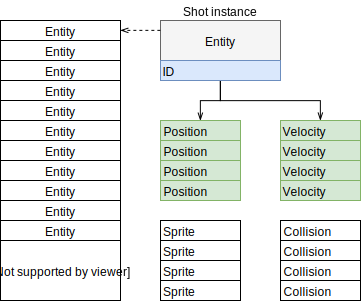
\includegraphics[width=0.7\linewidth]{BAC-DOC2}}
	\caption{Obsah paměti u~datově orientované kompozice. \emph{Identifikátor} jednoznačně mapuje entity na jednotlivé instance komponent.}
	\label{Fig:DOCMemory}
\end{figure}

Organizaci paměti, se kterou dále tento příklad parcuje, lze vidět na obr. \ref{Fig:DOCMemory}. Entity jsou uchovávány v~homogenním poli. Jednotlivé identifikátory entit je možné mapovat na komponenty přímou indexací polí komponent.

\begin{figure}[H]
	\centering
	\tmpframe{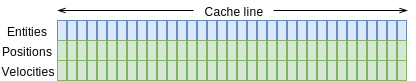
\includegraphics[width=0.7\linewidth]{BAC-DOC3}}
	\caption{Využití procesorové vyrovnávací paměti při použití datově orientované kompozice.}
	\label{Fig:DOCCache}
\end{figure}

Pro ukázku práce s~vyrovnávací paměti je opět použit příklad iterace nad seznamem entit, které je nutno posunout v~prostoru. Pro vykonání této akce je tedy nutný přístup ke komponentám typu \textbf{Position} a \textbf{Velocity}. Nejdříve je opět přistoupeno k~poli entit, čímž je načten příslušný řádek do vyrovnávací paměti. Jelikož je mapování identifikátorů entit realizováno pomocí přímé indexace\footnote{Za předpokladu, že identifikátory všech iterovaných entit nedovolují díry v~poli komponent.}, je možné po načtení řádku vyrovnávací paměti pro dané dva typy komponent již následující realizovat přímo z~paměti \emph{cache}. Obrázek \ref{Fig:DOCCache} obsahuje ilustraci stavu vyrovnávací paměti, po provedení první operace.

Komunikace mezi jednotlivými částmi je v~případě \emph{datově orientované kompozice} rozdělená do dvou úrovní. První z~nich, komunikace mezi komponentami, je vyřešena implicitně, jelikož akce mohou přistupovat k~několika komponentám. Druhou je potom komunikace mezi zprostředkovateli akcí (např. \emph{systémy}). Tento typ komunikace je možné opět řešit pomocí systému zpráv, nebo událostí. 

\noindent Mezi výhody \emph{DOC} patří: 
\begin{itemize}
	\item Efektivní skladování entit, které jsou reprezentovány identifikátorem.
	\item Lepší využití vyrovnávacích pamětí.
	\item Možnost definování nových typů entit za běhu, použitím kompozice.
	\item Odstraněna duplikace kódu a akumulace nechtěného stavu.
	\item Možnost efektivní implementace akcí, mimo komponenty.
	\item Opakované provádění jednoduchých akcí, nad seznamy komponent, umožňuje efektivní využití instrukční vyrovnávací paměti.
\end{itemize}

\noindent Její nevýhody jsou: 
\begin{itemize}
	\item Bez podpory v~programovacích jazycích \footnote{Vzniká programovací jazyk, který bude tento typ kompozice podporovat \cite{OOHLang}.}.
	\item Náročná implementace.
\end{itemize}

\noindent Mezi další vlastnosti patří:
\begin{itemize}
	\item Ztráta abstrakce při práci s~komponentami.
	\item Komponenty jsou čistá data, čímž je umožněna \emph{serializace} entit a komponent.
	\item Akce mohou přistupovat k~několika komponentám.
\end{itemize}

\section{Entity-Component-System}
\label{Chap:EntitySystem} 

Entitní systémy, postavené za použití \emph{datově orientované kompozice}, s~využitím \emph{systémů} pro implementaci chování, se nazývají \emph{Entity-Component-System}\footnote{Často používaným označením je také \uv{component base entity system},  \uv{Component-Entity-System}, nebo i \uv{Entity System}.}. Tato část obsahuje popis konceptů, se kterými tento typ entitního systému pracuje a vlastností, které z nich vyplývají.

\subsection{Motivace a koncepty}

\emph{Entity-Component-System} (\emph{ECS} \cite{WhatIsECS, UnderstandingECS}) je návrhové paradigma \cite{EntitySystemsFuture}, založené na kompozici a striktní separaci logiky (\emph{systémy}) a dat (\emph{entity}, \emph{komponenty}). \emph{ECS} vychází z principů \emph{datově orientovaného} návrhu, díky čemuž dokáže efektivně využívat moderní výpočetní hardware. Výsledný systém umožňuje vyšší úroveň modularity a~dynamické změny aplikace za běhu.

Entita je základním stavebním blokem \cite{EntitySystemsFuture}, který lze přirovnat k~objektu z~\emph{objektově orientovaného} návrhu. Na rozdíl od objektů nejsou však entity tvořeny z předem definovaného vzoru (např. třídy), ale jejich funkce -- chování a data -- je definována množinou komponent, které daná entita vlastní. Entity lze reprezentovat pomocí jednoznačných identifikátorů (čísel), které mají podobnou funkci, jako \emph{primární klíče} v~databázi, ilustrace tohoto přirovnání lze vidět na obr. \ref{Fig:ECSDB}.

\begin{figure}[H]
	\centering
	\tmpframe{\includegraphics[width=0.7\linewidth]{BAC-ECS1}}
	\caption{Entita reprezentována jako řádek v~databázi. Primárním klíčem je identifikátor entity.}
	\label{Fig:ECSDB}
\end{figure}

Komponenty jsou základními nosiči dat v~\emph{ECS}. Často používaným názvem pro komponenty, je také \uv{aspekt} \cite{EntitySystemsFuture}, jelikož po přiřazení komponent k~entitám mají komponenty další funkci -- určují množinu chování entit. Kromě explicitních dat obsažených v~komponentách existuje také, implicitní informace o~tom, zda daná entita obsahuje (má přiřazen) určitý typ komponenty. Každá entita má k~sobě přiřazeno 0 a více\footnote{Častým omezením, které se v reálných implementacích \emph{ECS} objevuje, je omezení maximálního počtu komponent na 1.} komponent daného typu, kde přítomnost komponenty znamená, že entita splňuje daný aspekt. V~přirovnání \emph{ECS} k~\emph{relační databázi}, lze o~komponentách smýšlet jako o~sloupcích (obr. \ref{Fig:ECSDB}) tabulky entit.

Pokud bychom pokračovali s~přirovnáním k~\emph{OOP} -- entity jsou jednotlivé objekty, komponenty umožňují polymorfizmus -- potom systémy implementují chování, nebo metody jednotlivých komponent. Pro mnoho různých typů dat, kde každý typ vyžaduje vlastní chování, je \emph{OOP} výhodné, protože je možné data i operace uložit do jednoho nerozdělitelného celku. Pokud je však nutné vykonat stejnou akci na velkém množství různých typů, \emph{OOP} není optimálním řešením a \emph{ECS} je v~tomto případě vhodnější \cite{EntitySystemsFuture}. 


\begin{figure}[H]
	\centering
	\tmpframe{\includegraphics[width=0.7\linewidth]{BAC-ECS3}}
	\caption{Filtr operuje nad entitou a informací o~přítomnosti komponent.}
	\label{Fig:ECSFilter}
\end{figure}

Každý systém provádí danou operaci na všech entitách, které obsahují požadované komponenty (\emph{aspekty}). Základní schéma systému lze vidět na obr. \ref{Fig:ECSSystem}. Výběr vhodných entity je proveden pomocí filtru, který operuje nad přítomností jednotlivých komponent (obr. \ref{Fig:ECSFilter}).

\begin{figure}[H]
	\centering
	\tmpframe{\includegraphics[width=0.7\linewidth]{BAC-ECS2}}
	\caption{Vstupem \emph{systému} jsou entity, ze kterých si vybere pouze ty, které mají odpovídající komponenty. Na vybraných entitách provádí požadované akce.}
	\label{Fig:ECSSystem}
\end{figure}

\subsection{Vlastnosti}

Důvodů, proč se \emph{ECS} používá při návrhu moderních her, je mnoho a většina z~nich vzniká díky striktnímu oddělení logiky a dat. Komponenty je možné skladovat v~sekvenčních blocích paměti, čímž je vylepšena efektivita využití vyrovnávacích pamětí. Lokalita dat se vztahuje i na instrukce\footnote{\emph{Instrukční cache} \cite{CpuMemoryGap, InstrAreData}} a díky opakovanému provádění stejných operací nad velkým počtem entit dochází k~vyšší efektivitě využití \emph{instrukční cache}. 

Inherentní modularita \emph{ECS} dovoluje lepší dělení práce ve velkých týmech vývojářů. Každý systém musí předem specifikovat, o~jaké entity (které aspekty musí splňovat) má zájem, tímto je zamezeno nechtěnému ovlivňování okolního kódu. Další výhodou, z~pohledu organizace kódu, je přímočará \emph{refaktorizace} systémů a komponent.

Jelikož komponenty obsahují pouze čistá data, bez propojení do externích modulů, je možné přistupovat k~entitnímu systému také z~vestavěného skriptovacího jazyka (např. \emph{LUA}). Skriptovací jazyky bývají hojně využívány jako součást \uv{gameplay}\footnote{Kód, který se stará o~interakce virtuálních objektů ve hře.} funkcí, nebo \emph{umělé inteligence}. Pokročilou vlastností \emph{ECS} může také být přidávání nových typů komponent za běhu aplikace. Tyto, ale i~další (např. \emph{serializace} komponent), funkce umožňují rychlé prototypování nových herních mechanik.

Při správném rozvržení systémů a jejich požadovaných aspektů, je možné zaručit, že k~ostatním komponentám nebude přistupováno. Tímto je umožněna vyšší úrovně paralelizace celého systému, přestože několik systémů může v~jeden čas přistupovat ke stejné entitě. Paralelizace je dále podporována opakovaným prováděním stejných akcí nad velkým množstvím entit, které lze rozdělit mezi jádra procesoru a~zpracovat je odděleně.

\section{Existující řešení}

Tato část obsahuje porovnání existujících knihoven, které umožňují práci s~entitními systémy založenými na \emph{ECS} paradigmatu. Kromě základního popisu jsou zde také uvedeny výhody a nevýhody daných přístupů. Mezi další známé knihovny pro tvorbu her, které používají komponentní přístup, patří \emph{Unity}, \emph{Unreal Engine}, nebo např. \emph{libGDX} (knihovna \emph{Ashley} \cite{Ashley})

\subsection{EntityX}

\textbf{EntityX} \cite{EntityX} je implementace entitního systému v~programovacím jazyce \emph{C++}, která silně využívá vlastností standardu \emph{C++11} a \emph{šablonového metaprogramování} \cite{CppMetaprogramming}. Toto umožňuje příjemnější práci s~typy, pro uživatele této knihovny. Entity jsou v~tomto případě nepřímo mapovány (pomocí identifikátorů) na komponenty, které jsou uloženy v~souvislých polích, což umožňuje efektivní využití vyrovnávací paměti. 

Kromě základní implementace entitního systému, podle \emph{ECS}, knihovna také umožňuje uživatelům knihovny reagovat, když entity \uv{vcházejí}, nebo \uv{vycházejí} do \emph{systémů}, čímž dovoluje entitní systém propojit s~okolním kódem.

Mezi hlavní nevýhody patří delší doba překladu výsledné aplikace -- výsledek použití šablon. Vlastnost, která je na jednu stranu výhodou, ale má i jisté nepříjemné stránky, je nemožnost registrace nových typů komponent za běhu aplikace. Výhodou je v~tomto případě možnost vyšší optimalizace výsledné přeložené aplikace.

\subsection{Artemis}

\textbf{Artemis} \cite{ArtemisJava} je původně knihovna implementovaná pro jazyk \emph{Java}, ale existuje i mnoho implementací pro další jazyky, např. \emph{C++} \cite{ArtemisCpp}. Knihovna využívá \emph{generického programování} jazyka \emph{Java}, čímž opět umožňuje uživateli příjemnější práci. Oproti ostatním knihovnám podporuje vyšší granularitu filtrování entit, kdy je možné specifikovat, které komponenty entita musí, může a nesmí obsahovat. Další zajímavou vlastností je speciální typ komponent -- značky -- které neobsahují žádná data, ale umožňují entity dělit do skupin. 

Knihovna také umožňuje využití pokročilých funkcí, jako sdružování entit a jejich tvorba ve vyšších počtech, nebo entitní \emph{archetypy}, které fungují jako předloha pro další entity.

Knihovna \textbf{Artemis} je ze všech představených knihoven nejvíce dokončená a existují již i projekty, které ji používají.

\subsection{Anax}

Kromě základní implementaci vlastností \emph{ECS}, obsahuje knihovna \textbf{Anax} \cite{Anax} také pojem \emph{skupin}. \emph{Skupiny} obsahují před generovaný seznam entit, skrz který \emph{systémy} iterují. Výhodou tohoto přístupu je možnost rychlé práce s~celým seznamem entit, které vyhovují určitému filtru. Mezi nevýhody patří nutnost tyto seznamy udržovat. Podobně, jako \textbf{EntityX}, je tato knihovna implementována v~jazyce \emph{C++}. 

\section{Paralelizmus}
\label{Chap:Parallelism}

Vývoj moderních procesorů se ubírá směrem zvyšování počtu výpočetních jader \cite{CPUPerfHistory} a proto i moderní aplikace musí být schopné tato jádra využít. To je zvláště pravda pro vývoj her, které se snaží s~hardware vytěžit maximální výkon. Paralelizace aplikací, jejichž části jsou úzce provázané je obzvláště problematické a proto vznikají nové způsoby tento typ software navrhovat -- jedním z~nich je právě \emph{ECS}. 

Paralelizmus lze obecně rozdělit na 2 typy -- datový a úkolový \cite{KindsOfParallelism}. Při použití datového paralelizmu je prováděna jedna akce, na různých datech (obdoba \emph{SIMD} u~procesorů). Opačným přístupem je paralelizmus úkolový \cite{TaskBasedParallelism}, u~kterého mohou běžet různé operace nad stejnými daty (\emph{MISD}). Ve většině případů je však používáno kombinací těchto dvou přístupů. Speciálním případem je vyhrazení celého vlákna jednomu modulu -- např. manažer zvuku -- který vyžaduje nízké odezvy \cite{FrontierThreads}.

Výhodou paralelizmu je možnost rozložení práce na několik výpočetních jednotek, což umožňuje požadovanou akci provést rychleji. Využití paralelizmu však představuje mnoho nových typů problémů, které se u~sekvenčního programování nevyskytují. Kromě obecně známých překážek, jako jsou synchronizace vláken, potenciální uváznutí (\emph{deadlock}), různých typů souběhu (\emph{race condition}), existují také problémy na hardwarové úrovni. Hlavním z~nich je udržování koherence procesorových \emph{cache} \cite{CacheCoherence} a skrz to problém, který se nazývá \uv{false sharing} \cite{FalseSharing}. V~případě, že několik vláken pracuje se stejným blokem paměti -- je načtený v~jeho lokální vyrovnávací paměti -- je nutné \emph{cache} jednotlivých jader synchronizovat tak, aby každé z~nich nepracovalo s~jinými daty. Tento proces se nazývá \uv{udržování koherence vyrovnávacích pamětí}. Problém, který v~tomto systému může nastat -- \uv{false sharing} -- vzniká v~případě, kdy obě vlákna pracují nad stejnou pamětí \footnote{Paměť je součástí stejného řádku vyrovnávací paměti.}, ale nepracují se stejnými daty. Při každé změně bude nutno provést synchronizaci, i když není nutná, ilustraci tohoto jevu lze vidět na obr. \ref{Fig:PARFalseSharing}.

\begin{figure}
	\tmpframe{\includegraphics[width=\linewidth]{BAC-PAR0}}
	\caption{Udržování koherence vyrovnávací paměti a \uv{false sharing} \cite{FalseSharing}. Synchronizace \emph{cache} je prováděna mezi jednotlivými jádry, přes specializovanou sběrnici.}
	\label{Fig:PARFalseSharing}
\end{figure}

\emph{Entity-Component-System} paradigma je výhodné z~pohledu více-jádrových systémů, díky možnosti téměř \cite{AmdahlLaw} dokonalé paralelizace na několika úrovních \cite{ParallelGame}. První úrovní paralelizace, kterou \emph{ECS} umožňuje, je datový paralelizmus, kde se uvnitř systému množina všech entit, které odpovídají požadavkům, rozdělí do množiny vláken, které mohou dané akce provádět odděleně \footnote{Některé typy akcí tento paralelizmus neumožňují - např. výpočet pozic objektů v~grafu scény.}. Ilustrace principu, jak tento způsob pracuje lze vidět na obr. \ref{Fig:PARData}. Dalším způsobem paralelizace je možnost spouštět jednotlivé systémy na oddělených vláknech (obr. \ref{Fig:PARSystem}), tato metoda je ovšem použitelná pouze pro systémy, které nezapisují do komponent, které jsou zároveň používány v~jiném systému. 

\begin{figure}
	\tmpframe{\includegraphics[width=\linewidth]{BAC-PAR1}}
	\caption{Paralelizmus uvnitř systémů je příkladem datového paralelizmu \cite{KindsOfParallelism}.}
	\label{Fig:PARData}
\end{figure}

\begin{figure}
	\tmpframe{\includegraphics[width=\linewidth]{BAC-PAR2}}
	\caption{Paralelizmus na úrovni systémů, kdy několik systémů běží zároveň.}
	\label{Fig:PARSystem}
\end{figure}

Jednoduchý systém může pracovat způsobem transformační funkce, jejíž vstupní parametry jsou komponenty, které systém požaduje a výstupem je zápis (změna) jedné z~těchto komponent. Jelikož je ovšem vhodné, při paralelním přístupu k~aktuálnímu stavu herního světa, aby všechny systémy dokázaly přečíst původní data beze změn, lze funkci systémů změnit. Systémy mohou místo zápisu nových hodnot do stejných komponent (vstupů) zapsat výsledek do \uv{následujícího stavu} \cite{FrontierThreads} \footnote{Tento způsob je často používán ve funkcionálních jazycích.}. Při generování nového stavu je nutné určit okamžik, kde se následující stav stane stavem aktuálním, čímž se celý herní svět \uv{posune}.

\chapter{Návrh entitního systému}
\label{Chap:Design}

Obsahem této kapitoly je popis návrhu entitního systému založeného na \emph{ECS} paradigmatu, které bylo představeno v~předchozí kapitole. Nejdříve je prezentováno základní rozdělení systému na jednotlivé části a komunikace mezi nimi. Následuje popis návrhu podsystémů -- \emph{komponenty}, \emph{systémy} a \emph{entity}. Každá část obsahuje představení návrhu a jeho zdůvodnění. Následuje návrh paralelního přístupu k~entitnímu systému a jeho tok řízení.

Při návrhu entitního systému byly použity poznatky z~teoretické části této práce a \emph{open-source} implementace entitních systémů založených na \emph{ECS} paradigmatu -- \emph{EntityX} \cite{EntityX}, \emph{ArtemisCpp} \cite{ArtemisCpp}, \emph{Anax} \cite{Anax}, \emph{Artemis} \cite{ArtemisJava} a \emph{Ashley} \cite{Ashley}.

\section{Přehled a komunikace}

Entitní systém je, podobně jako \emph{ECS} paradigma, rozdělený do několika částí -- modulů -- kde cílem jednotlivých částí je správa některé z~domén \emph{ECS}. Diagram reprezentující toto rozdělení lze vidět na obr. \ref{Fig:DESModules}. Mezi tyto moduly patří -- správa systémů a skupin, správa komponent, správa entit a správa akcí. Bližší popis a návrh jednotlivých částí obsahují následující části této kapitoly.

\begin{figure}[H]
	\tmpframe{\includegraphics[width=\linewidth]{BAC-DES1}}
	\caption{Rozdělení entitního systému do modulů.}
	\label{Fig:DESModules}
\end{figure}

Funkcionalita celého systému je zastřešena třídou \textbf{Universe} (obr. \ref{Fig:DESUniverse}), skrz kterou je uživateli umožněn přístup k~jednotlivým podsystémům. Pro každou operaci nad entitním systémem existuje metoda uvnitř třídy \textbf{Universe} -- tento návrh umožňuje jednotný vstupní bod. Nevýhodou je vysoké množství metod v~této třídě. Další důležitou funkcionalitou třídy \textbf{Universe} je zprostředkování komunikace mezi jednotlivými moduly -- např. přidání komponenty má dvě části, skutečná operace nad nosičem komponent a úpravu metadat (obr. \ref{Fig:DESAddComp} a obr. \ref{Fig:DESAddEnt}). 

\begin{figure}[H]
	\tmpframe{\includegraphics[width=\linewidth]{BAC-DES2}}
	\caption{Třída \textbf{Universe} je rozhraním entitního systému. Diagram neobsahuje specifikaci všech metod třídy, kvůli jejich vysokému počtu.}
	\label{Fig:DESUniverse}
\end{figure}

\section{Komponenty a jejich nosiče}

Komponenty jsou definovány jako základní datové jednotky v~\emph{ECS}, kde každá entita má k~sobě přiřazeno 0-1 komponent daného typu. Komponenty, jak s~nimi pracuje tento návrh, mohou být jakékoliv třídy \footnote{Obecný typ komponenty je \textbf{Component}. Pokud to implementační jazyk vyžaduje, je možné požít abstraktní třídu stejného jména, ze které budou všechny konkrétní komponenty dědit.} a nemusí obsahovat žádné specifické akce. Každá komponenta má přiřazen unikátní identifikátor -- \textbf{CompId} -- tento identifikátor je neměnný po dobu běhu entitního systému. Komponenty by měly být pasivní datové struktury \footnote{\emph{Plain old data structure} (\emph{POD}) -- struktura reprezentovaná kolekcí hodnot.}, se kterými lze pracovat jako s~čistou pamětí (přesuny, kopírování, atp.).

O~správu komponent se stará podsystém správy komponent, jehož diagram lze vidět na obr. \ref{Fig:DESCompDiag}. Modul se skládá dvou částí -- registrace typů komponent a nosiče komponent. Veškerá komunikace probíhá skrz třídu \textbf{Component Manager}, která obsahuje metody pro registrace komponent a jejich následná asociace k~entitám. 

V~první fázi práce s~tímto modulem je třeba registrovat typy komponent, které budou následně používány. Nové komponenty jsou registrovány pomocí metody \textbf{registerComponent} \footnote{Této metodě je třeba předat typ komponenty, která má být registrována, čehož lze docílit pomocí např. \emph{template} (C++), nebo \emph{generics} (Java)}, která vytvoří mapování z~daného typu na jeho registr (\textbf{ComponentRegister}). Tohoto registru je následně využito pro získání specifického nosiče komponent.

\begin{figure}[H]
	\tmpframe{\includegraphics[width=\linewidth]{BAC-DES5}}
	\caption{Diagram tříd podsystému správy \emph{komponent}.}
	\label{Fig:DESCompDiag}
\end{figure}

Každý typ komponent je uložen ve vlastním kontejneru -- tzv. nosič komponent. Nosičem je třída, která dědí z~\textbf{BaseComponentHolder} a implementuje všechny požadované operace, přičemž si může každá komponenta zvolit typ nosiče \footnote{Opět pomocí mechanizmu \emph{template}, nebo obdobných vlastností jiných jazyků.}. Hlavní funkcí nosiče je mapování identifikátorů entit (\textbf{EntityId}) na přiřazené komponenty. 

Různé implementace nosičů, specifické pro určené komponenty, umožňují vyšší úroveň optimalizace pro předpokládané využití komponent. Pokud je např. jisté, že téměř všechny entity budou obsahovat určitý typ komponenty, je možné implementovat nosič jako jednoduché pole, kde mapovací funkcí je prostá indexace komponent pomocí identifikátoru entit. Naopak, pokud je předpokladem, že komponenta bude využívána nízkým počtem entit, nosič může být implementován jako strom, kde klíčem je identifikátor entity. Speciálním typem komponenty je \emph{značka} (\emph{tag}), která neobsahuje žádná data, ale vzniká implicitní informace o~tom, zda má entita danou značku přiřazenu, čehož lze využít pro např. rozdělení entit do skupin.

\begin{figure}[H]
	\tmpframe{\includegraphics[width=\linewidth]{BAC-DES8}}
	\caption{Sekvenční diagram přidání komponenty, pokračuje na obr. \ref{Fig:DESAddEnt}.}
	\label{Fig:DESAddComp}
\end{figure}

Operace přidání komponenty je rozdělena do dvou částí, první z~nich, která pracuje nad \textbf{ComponentManager} lze vidět na obr. \ref{Fig:DESAddComp}. Po úspěšném přidání komponenty následuje modifikace metadat, kterými se zabývá následující část kapitoly o~návrhu.

\section{Reprezentace entit}

Entita, jako koncept z~\emph{ECS}, je distribuovaný objekt, složený z~komponent. Pro každou entitu existuje 1-0..1 mapování na každý typ komponent. Vyvstává tedy požadavek ne jednoznačný identifikátor entit, který by plnil funkci \emph{primárního klíče} v~tabulce (obr. \ref{Fig:ECSDB}) entit.

Pro účely tohoto entitního systému je identifikátor složen ze dvou čísel -- ID a generace. ID je v~tomto případě skutečný \emph{primární klíč}, pomocí kterého jsou jednotlivé řádky v~tabulce entit indexované \footnote{Používá se tedy i při mapování komponent na entity uvnitř nosičů komponent.}. Generační číslo odlišuje různé generace entit, které zabíraly stejný řádek v~tabulce (stejné ID) a je inkrementováno při každém smazání entity. Generační čísla identifikátorů, skrz které je přistupováno k~systému jsou porovnány s~aktuální generací dané entity, čímž je zamezen přístup ke smazaným entitám.

\begin{figure}[H]
	\tmpframe{\includegraphics[width=\linewidth]{BAC-DES6}}
	\caption{Diagram tříd podsystému správy \emph{entit}.}
	\label{Fig:DESEntityDiagram}
\end{figure}

Podsystém správy entit, jehož diagram tříd lze vidět na obr. \ref{Fig:DESEntityDiagram}, lze přirovnat k~relační databázi. Systém obsahuje jednu tabulku entit, kde každý řádek reprezentuje slot pro entitu. Identifikátor entity je složen z~indexu řádku v~tabulce a jeho generační hodnoty. Každý řádek obsahuje aktuální číslo generace a množinu \emph{bool} hodnot -- metadat. Ilustraci možné konfigurace tabulky metadat lze vidět na obr. \ref{Fig:DESMetadata}. Výhodou této reprezentace je konstantní složitost přístupu k~metadatům dané entity \footnote{Indexace tabulky pomocí \emph{ID} části identifikátoru.}. 

Jelikož je mapováni identifikátorů entit na komponenty již součástí nosičů komponent, tabulka již tuto informaci nemusí obsahovat. Výhodné je však udržování informace o~existenci komponent pro jednotlivé entity, které může být použito pro efektivní filtrování entit. Udržování tohoto typu informace je možné díky jednotnému rozhraní pro práci s~komponenty (\textbf{Universe}). Mezi typy metadat použitých v~tomto návrhu patří: 
\begin{itemize}
	\item Aktivita -- Entita může být ve stavu aktivní, nebo neaktivní.
	\item Obsazenost -- řádek je použitý, nebo prázdný. 
	\item Přítomnosti každého registrovaného typu komponent.
	\item Přítomnost entity ve skupinách \footnote{Více o~skupinách je součástí části. \ref{Chap:SysGroup} .}.
\end{itemize}

\begin{figure}
	\tmpframe{\includegraphics[width=\linewidth]{BAC-DES11}}
	\caption{Tabulka metadat, indexy jednotlivých entit jsou implicitní indexy řádků.}
	\label{Fig:DESMetadata}
\end{figure}

Důležitou součástí \emph{ECS} je možnost pracovat pouze s~entitami, které mají požadované komponenty (\uv{aspekty}). Z~tohoto důvodu je součástí správy entit i možnost filtrování (třída \textbf{EntityFilter}). Filtrovat lze pomocí seznamu požadovaných komponent, ale je také možno definovat zakázané komponenty, nebo specifikovat požadovanou úroveň aktivity entit (aktivní/neaktivní).

Poslední částí podsystému správy entit je třída \textbf{Entity}, jejíž funkcionalita zjednodušuje práci s~\emph{ECS}. Operace na ní provedené jsou pouze přesměrovány na \textbf{Universe}, spolu s~příslušným identifikátorem entity. Pomocí této třídy lze také \emph{ECS} propojit s~okolním \emph{objektově orientovaným} kódem.

\begin{figure}[H]
	\centering
	\tmpframe{\includegraphics[width=.6\linewidth]{BAC-DES10}}
	\caption{Sekvenční diagram modifikace metadat při přidání komponenty, pokračování obr. \ref{Fig:DESAddComp}.}
	\label{Fig:DESAddEnt}
\end{figure}

Nevýhodou udržování informací o~přítomnosti komponent na dvou místech je, že při každé změně je nutné, aby byla provedena i v~metadatech. Příkladem tohoto problému je operace přidání komponenty, jejíž sekvenční diagram lze vidět na obr. \ref{Fig:DESAddComp}. Pokud je první fáze (přidání komponenty z~pohledu \textbf{Component Manager}) úspěšná, je nutné upravit metadata.

\section{Systémy a skupiny}
\label{Chap:SysGroup}

\emph{Systém}, podle \emph{ECS} paradigmatu, obsahuje pravidla pro výběr vhodných entit a akce, které na nich provádí. Entity jsou filtrováni pomocí množiny požadovaných komponent (aspektů). Vstupem \emph{systému} je tedy seznam entit, které vyhovují filtračním pravidlům a jeho cílem je transformovat dané entity a jejich komponenty pomocí definované akce. Tato myšlenka je základem podsystémy správy \emph{systémů}. 

Předpokladem, při návrhu tohoto entitního systému je, že i přeš vysoký počet entit, které se v~systému mohou nacházet v~jeden okamžik, bude množství skutečně používaných entit \footnote{Těch, které budou používány jako součást některého ze systémů.} nižší. Z~tohoto předpokladu vychází myšlenka \emph{skupin}, které jsou plní funkcí vyrovnávací paměti \emph{systémů}. \emph{Skupina} je množinou entit, které splňují požadavky specifikované filtrem. Oproti původnímu návrhu, kdy každý \emph{systém} iteruje (lineárně prochází) nad seznamem všech existujících entit v~entitním systému, se při použití skupin již prochází pouze takové entity, které odpovídají požadavkům daného systému.

Jednou z~nevýhodou použití \emph{skupin} je nutnost skupiny udržovat aktuální, čímž je pověřen podsystém správy \emph{skupin}. Díky potřebě udržování seznamu entitních identifikátorů způsobuje tento systém také vyšší použití paměti. Poslední důležitou vlastností je, že tato funkce předpokládá, že množina všech entit je větší, než množina používaných entit. Pokud tento předpoklad neplatí, potom není vhodné systém \emph{skupin} používat.

\begin{figure}[H]
	\centering
	\tmpframe{\includegraphics[width=.7\linewidth]{BAC-DES3}}
	\caption{Diagram tříd podsystému správy \emph{systémů}.}
	\label{Fig:DESSystemDiagram}
\end{figure}

Cílem podsystému správy \emph{systému} (obr. \ref{Fig:DESSystemDiagram}), je údržba systémů a jejich vazba na skupiny. Třída \textbf{SystemManager} umožňuje přidávání a odběr nových systémů. \emph{Systémy} jsou definovány uživatelem, ktery vytvoří vlastní třídu, která dědí ze základní třídy \textbf{System}. Dále uživatel musí specifikovat požadované vlastnosti entit -- vyžadované / zakázané komponenty a úroveň aktivity. Následně je možné nový typ \emph{systému} přidat pomocí manažerské třídy. 

\begin{figure}[H]
	\centering
	\tmpframe{\includegraphics[width=.7\linewidth]{BAC-DES4}}
	\caption{Diagram tříd podsystému správy \emph{skupin}.}
	\label{Fig:DESGroupDiag}
\end{figure}

\emph{Skupiny} (\textbf{EntityGroup}) obsahují 3 seřazené seznamy entitních identifikátorů, jejich významy jsou následující -- přidané entity, odebrané entity a skutečný seznam všech vyhovujících entit. Důvod pro existenci prvních dvou je primárně umožnit uživateli propojit entitní systém se systémy okolními, které (např. fyzikální simulace) potřebují objekty registrovat.

Důležitou vlastnosti \emph{skupin} je možnost přidávat a odebírat je za běhu aplikace \footnote{Některé systémy nemusí zpracovávat entity po celý běh aplikace.}. Tato vlastnost je umožněna skrz podsystém správy \emph{skupin} (\ref{Fig:DESGroupDiag}). Každá \emph{skupina} obsahuje \uv{počítadlo referencí}, které reprezentuje na kolika různých místech je \emph{skupina} používána. V~případě, že počítadlo dosáhne hodnoty 0, je \emph{skupina} odstraněna (nebo je pouze zastaven její běh). Zpráva \emph{skupin} závisí na entitních metadatech, které umožňují efektivnější aktualizace jejich obsahu \footnote{Více o~tomto problému je součástí implementační části \ref{Chap:ImplSystem}.}.

\section{Paralelní přístup}

Díky modulárnímu návrhu entitního systému, který byl zatím předveden je implementace základních typů paralelního přístupu velmi přímočará. Mezi základní typy paralelizmu, který entitní systém podporuje jsou paralelizmus na úrovni entit a paralelizmus na úrovni systému.

Paralelizmus na úrovni entit využívá \emph{datového paralelizmu}, kde množina entit, nad kterou systém vykonává akce je rozdělena mezi požadovaný počet paralelních vláken. Tento typ paralelizmu je vhodný pouze v~případech, kdy akce vykonávají transformace na entitách (a jejich komponentách), bez potřeby informací z~ostatních entit. 

Paralelizmus na úrovni systémů lze přirovnat k~\emph{úkolovému paralelizmu}, kde každé vlákno zpracovává rozdílný systém. Tento způsob má opět omezení -- systémy nemohou přistupovat ke stejným komponentám (stejných entit). Tyto dva způsoby paralelizmu lze kombinovat.

V~situacích, kdy není možné použít ani jednu z~těchto možností, nebo při manipulaci globálního kontextu z~několika vláken, např. mazání entit, změna aktivity, je nutné použít jiné řešení. Jedním způsobem, jak tento problém vyřešit, je použití zámků (např. vzájemné vyloučení -- \uv{mutex}), které budou tyto metody chránit před problémy souběhu (\uv{race condition}). Zámky jsou čistým způsobem, jak implementovat bezpečný paralelizmus, ale vysokém počtu operací zamčení a odemčení je možné ztratit výkon, který byl získán paralelním zpracováním \footnote{Pokud jsou operace chráněné zámky používány často, je možné paralelní aplikaci redukovat na aplikaci sekvenční.}. Kvůli těmto nevýhodám je součástí návrhu také třetí metoda paralelizace -- pomocí \emph{množin změn}.

\emph{Množiny změn} umožňují jednotlivým vláknům odkládat provedení požadovaných operací na pozdější dobu, kdy již bude možné zaručit, že nedojde k~problémům souběhu. Aktuální stav světa (entit, komponent apod.), pro každé vlákno, je vytvořen překrytím stavu globálního světa danou \emph{množinou změn}. Pokud vlákno použije operaci přidání komponenty, ke specifikované entitě, skutečné vykonání operace nad globálním kontextem bude odloženo, ale informace o~této operaci bude přidána do \emph{množiny změn} aktuálního vlákna.

\begin{figure}[H]
	\tmpframe{\includegraphics[width=\linewidth]{BAC-DES7}}
	\caption{Diagram tříd podsystému správy \emph{akcí}.}
	\label{Fig:DESActionDiag}
\end{figure}

Základem podsystému \emph{množin změn}, jehož diagram lze vidět na obr. \ref{Fig:DESActionDiag}, jsou třídy \textbf{ActionCache} a textbf{ChangeSet}. Úkolem \textbf{ActionCache} je zajistit přístup k~instanci \emph{množin změn}, která bude pro každé vlákno unikátní. Dále umožňuje také potvrzení (\textbf{commitSC}), nebo zrušení (\textbf{resetCS}) \emph{množiny změn} aktuálního vlákna. 

Zajímavým problémem je odložená tvorba entit a následné provádění operací nad nimi. Pro operace, které jsou provedeny nad \emph{reálnými} entitami \footnote{Takové entity, které jsou již vytvořeny v~globálním kontextu.} je možno specifikovat cílovou entitu pomocí jejího identifikátoru. Jedním možným řešením je zakázat provádění operací nad dočasnými entitami, nebo zrušit koncept dočasných entit kompletně a provádět operace vytvoření entity okamžitě \footnote{Toto by znamenalo použití zámků na celý podsystém správy entit a metadat.}. Druhým řešením, které je součástí tohoto návrhu, je přiřazení speciálního typu identifikátoru dočasným entitám, který bude později převeden na identifikátor reálné entity. Operace, jejíž provedení je odloženo na později, mají postfix \uv{\textbf{D}} (\uv{deferred}) a operace, které pracují s~dočasnými entitami jsou zakončeny \uv{\textbf{T}} (\uv{temporary}).

\emph{Množiny změn} samotné jsou reprezentovány třídou \textbf{ChangeSet}, která obsahuje odložené \emph{akce}. \emph{Akce} je možno rozdělit na typy podle změn:
\begin{itemize}
	\item Změny metadat -- rušení entit, změna aktivity entit.
	\item Změny komponent -- přidání/odebrání komponent, změna hodnot komponent.
\end{itemize}
\noindent a podle cílové entity: 
\begin{itemize}
	\item Reálné entity -- operace obsahuje identifikátor reálné entity.
	\item Dočasné entity -- operace obsahuje identifikátor dočasné entity.
\end{itemize}

\section{Tok řízení}

Výše navržený entitní systém se vždy nachází v~jedné z~následujících fází -- \emph{inicializace}, \emph{iterace} nebo \emph{obnova}. Diagram řízení toku, který tyto fáze obsahuje, lze vidět na obr. \ref{Fig:DESFlow}.

\begin{figure}[H]
	\begin{center}
	\tmpframe{\includegraphics[width=0.9\linewidth]{BAC-DES9}}
	\end{center}
	\caption{Digram toku řízení komponentního systému.}
	\label{Fig:DESFlow}
\end{figure}

Prvním krokem ve fázi inicializace je konstrukce (vytvoření instance) třídy \textbf{Universe}, jejíž součástí je inicializace jednotlivých podsystémů. Potom je již možno registrovat typy komponent, které je potvrzeno závěrečnou inicializací objektu \textbf{Universe} \footnote{Po inicializaci již není možno přidávat nové typy komponent.}, čímž se entitní systém přesunuje do fáze \emph{iterace}. 

Fáze \emph{iterace} umožňuje plný přístup k~entitnímu systému ze strany uživatele. Kromě práce s~entitami a komponentami, je také možné přidávat a odebírat \emph{systémy} a \emph{skupiny}. Obsah jednotlivých \emph{skupin} je v~této fázi konstantní, čímž je umožněna práce \emph{systémům}. V~okamžiku, kdy již neběží žádné \emph{systémy} je možné přejít do fáze \emph{obnovy}, použitím operace \textbf{refresh}.

Úkolem \emph{obnovovací} fáze je posunutí entitního systému do následujícího stavu, ze stavu aktuálního a dokončení operací, které by vedly k~porušení konzistence systému. Tohoto cíle je dosaženo postupným voláním operace \textbf{refresh} na jednotlivé podsystémy, jejichž pořadí lze vidět na obr. \ref{Fig:DESFlow}. Obnova entitního podsystému umožňuje dokončení operací přidání a odebrání \emph{skupin}, u~kterých je nutné měnit počet sloupců v~tabulce metadat. Následuje aplikace \emph{množin změn}, kdy jsou dokončeny odložené operace. Obnova pokračuje volání \textbf{refresh} nad jednotlivými nosiči komponent, kterým je tímto umožněna reorganizace dat. Poslední částí je příprava obsahu \emph{skupin} pro příští fázi \emph{iterace}. Po dokončení obnovy je systém opět uveden do fáze \emph{iterace}.

\chapter{Implementace}
\label{Chap:Implementation}

Tato kapitola obsahuje popis implementace výše popsaného návrhu entitního systému, založeného na \emph{ECS} paradigmatu, přičemž jsou zde zmíněny pouze zajímavější implementační detaily. V~první části je zdůvodněn výběr implementačního jazyka a použitých knihoven. Následují části zaměřené na jednotlivé podsystémy entitního systému -- \emph{komponenty}, \emph{entity} a \emph{systémy}. Závěr kapitoly je zaměřen na implementaci paralelního přístupu a \emph{obnovovací} fázi. Výsledným produktem této implementace je knihovna, která umožňuje práci s~entitním systémem za využití \emph{ECS} paradigmatu. 

Dosavadní návrh entitního systémy lze shrnout do tří částí. První z~nich je správa komponent, kde komponenty jsou základní datové bloky, ze kterých se dále skládají entity. Komponenty jsou uchovávány v~\emph{nosičích} komponent, které zprostředkovávají mapování entit na jejich komponenty. Druhou částí entitního systému jsou entity samotné. Entita je definována identifikátorem, který jednoznačně určuje danou entitu. Identifikátor je složen ze dvou částí -- index a generace. Poslední částí jsou \emph{systémy}, které provádějí akce nad entitami. \emph{Systém} je složen z~definice entit, o~které má zájem -- které komponenty entita má obsahovat -- a z~akce, kterou nad vybranými entitami provádí. Součástí správy \emph{systémů} jsou také \emph{skupiny}, které operují jako vyrovnávací paměť a obsahují seznam entit pro daný \emph{systém}. 

\section{Implementační nástroje a přenositelnost}

Pro implementaci byl zvolen programovací jazyk \emph{C++} \cite{IsoCpp}, ve standardu \emph{C++14} \cite{Cpp14}. Jazyk \emph{C++} byl vybrán díky jeho dlouhodobému používání v~herním průmyslu, jako primární implementační jazyk mnoha herních \emph{enginů}. Mezi jeho další výhody patří optimalizované překladače, nebo možnosti výběru z~několika programovacích paradigmat. Jazyk byl použit ve standardu \emph{C++14}, který kromě ulehčení práce s~typy obsahuje také možnosti použití \emph{šablon proměnných} (\emph{variable templates} \cite{Cpp14VarTemplate}). 

Další důležitou vlastnosti, která byla zvážena při výběru implementačního jazyka, je přenositelnost vytvořené knihovny na různé hardwarové architektury a operační systémy. Díky standardu \emph{C++} je možné psát přenositelný kód, který je následně přeložen na specifické instrukce pro cílovou platformu a výsledné chování aplikace j stejné \footnote{Překlad knihovny byl testován za použití překladačů \emph{GCC}, \emph{Clang} a \emph{MSVC}, více ke specifikaci testovacích systémů lze najít v~kapitole \ref{Chap:Results}.}. 

Pro implementaci entitního systému byly použity pouze standardní knihovny jazyka \emph{C++}, čímž jsou zmírněny potenciální komplikace při používání výsledné knihovny. Při vývoji bylo také použito \emph{šablonového metaprogramování} \cite{CppMetaprogramming}, které umožňuje práci s~typy.

\section{Komponenty}

Komponenty lze definovat jako třídy (nebo struktury), pro která platí určitá omezení. Prvním z~nich je požadavek, aby komponenta obsahovala pouze data, která lze kopírovat jako čistou paměť (\emph{POD}), jelikož volání konstruktorů a destruktorů není zaručeno. Komponenta může obsahovat konstruktory, které inicializují data na jejich požadovanou hodnotu, ale vždy musí existovat výchozí konstruktor \footnote{Konstruktor bez parametrů.}. Komponenty také mohou specifikovat, který nosič by měl být použit pro jejich uchovávání \footnote{Pokud není specifikován, je použit výchozí nosič.}. Typ nosiče je definován v~zanořeném typu s~názvem \textbf{HolderT}.

Registrace komponent je prováděna pomocí statických šablon proměnných, kde pro každý typ komponent je vytvořena při překladu \footnote{Díky tomu, že jsou registry statické proměnné.} instance typu \textbf{ComponentRegister} (diagram na obr. \ref{Fig:DESCompDiag}). Tento registr obsahuje kromě informací o~komponentě také instance jejího nosiče. Díky \emph{šablonovému metaprogramování} je možné přímé mapování komponenty na instanci jejího nosiče za překladu programu, což umožňuje překladači vyšší úroveň optimalizace.

Knihovna obsahuje několik typů základních nosičů komponent. Prvním z~nich je implementace využívající standardní mapu (\textbf{std::map}), která mapuje identifikátory entit přímo na instance jednotlivých komponent. Tento typ nosiče je výhodný pro komponenty, které nejsou příliš často používané. Dalším krokem je nosič, který obsahuje souvislé pole komponent a mapu, která umožňuje mapování identifikátoru entity na index do pole komponent. Tento nosič je výhodný v~případech, kdy komponenty stále nejsou příliš časté, ale jsou zpracovávány v~blocích. Poslední typ nosiče je implementován jako čisté pole komponent, kde je mapování prováděno přímou indexací, pomocí identifikátoru entity. Výhodou je konstantní složitost přístupu k~jednotlivým komponentám, nevýhodou potom paměťová náročnost v~případě, kdy daný komponent neobsahuje každá entita. 

Uživatelům knihovny je umožněna implementace vlastních nosičů komponent, vytvořením vlastní třídy, která dědí ze základní třídy \textbf{BaseComponentHolder}. Jelikož informace, zda entita obsahuje daný komponent, je zpravována podsystémem entit, je velmi jednoduché implementovat např. nosič značek \footnote{Značka je komponent, který neobsahuje žádná data.}. 

\section{Správa entit}

Entity jsou definované pomocí identifikátorů, složených ze dvou částí -- index a generace. Index určuje číslo řádku v~tabulce entit a je také používán pro mapování komponent na entity. Generace určuje specifickou entitu, která \uv{obývá} daný řádek tabulky entit. Tento identifikátor je implementovaný jako třída \textbf{EntityId}, která, na rozdíl od návrhu, obsahuje pouze jedno číslo, rozdělené pomocí bitových operací do dvou částí (obr. \ref{Fig:IMPLIdent}). Ve výchozím nastavení knihovny je identifikátor reprezentován 32-bitovým číslem bez znaménka, indexová část zabírá 24 bitů a generace 8 bitů \footnote{Tato nastavení lze změnit v~hlavičkovém souboru.}. Validní identifikátor obsahuje indexové číslo, které není rovné nule. Speciálním případem identifikátoru je identifikátor dočasné entity, jehož generační číslo je rovno maximální hodnotě (255 pro výchozí nastavení).

\begin{figure}[H]
	\begin{center}
		\tmpframe{\includegraphics[width=\linewidth]{BAC-IMPL1}}
	\end{center}
	\caption{Rozdělení identifikátoru entit na generaci a index.}
	\label{Fig:IMPLIdent}
\end{figure}

Informace o~entitách je uložena v~tabulce entit, která obsahuje -- aktuální generaci, přítomnost komponentů, přítomnost entity ve skupinách, aktivitu a informaci o~tom, zda je daný řádek použitý. Až na generaci lze všechny informace reprezentovat jedním bitem, který je vždy ve stavu '1' (\emph{true}) nebo '0' (\emph{false}). Jelikož standardní množina bitů (\textbf{std::bitset}) nezaručuje uložení bitů v~souvislé paměti, vznikla za tímto účelem třída \textbf{InfoBitset}. Kromě souvislého uložení paměťových bloků, které obsahují jednotlivé bity, má \textbf{InfoBitset} další výhodu v~tom, že výše zmíněné paměťové bloky jsou uloženy ve třídě samotné a tudíž je možné její instance přesouvat pomocí operací s~pamětí (\emph{std::memcpy} atp.).

\begin{figure}[H]
	\begin{center}
		\tmpframe{\includegraphics[width=\linewidth]{BAC-IMPL2}}
	\end{center}
	\caption{Implementace tabulky metadat pomocí množin bitů \textbf{InfoBitset}. Tabulka obsahuje následující informace -- komponenty, skupiny, aktivitu, použití řádku a generaci. Z~této množiny informací jsou všechny, až na generaci, reprezentovány pomocí množin bitů.}
	\label{Fig:IMPLMetadata}
\end{figure}

Existují dva způsoby, jak organizovat jednotlivé bitové množiny -- horizontálně a vertikálně, ilustraci lze vidět na obr. \ref{Fig:IMPLMetadata}. Horizontální tabulka metadat obsahuje jednotlivé sloupce v~bitech stejné množiny bitů, na rozdíl od vertikální tabulky metadat, kdy pro každý typ metadat (např. každý typ komponent) existuje oddělený sloupec množin bitů. 

Mezi výhody horizontálního ukládání metadat patří jednodušší implementace a rychlejší filtrování \footnote{Filtrování je v~tomto případě pouze bitová operace \emph{AND}.}. Velkou nevýhodou je však problematický paralelní přístup k~jednotlivým bitům, jelikož není možné zaručit atomické bitové operace -- operace nad jedním bitem ovlivňují celý blok bitové paměti. 

Vertikální metadata naopak umožňují paralelní přístup k~odděleným sloupcům, díky čemuž je také použita ve finální implementaci této knihovny. Středem tabulky je třída \textbf{MetadataGroup}, která umožňuje udržovat skupinu sloupců metadat. Sloupce tabulky metadat jsou rozděleny do tří skupin -- komponenty, skupiny a ostatní. Skupina ostatních metadat obsahuje aktivitu entit a využitelnost řádku.

Operace vytvoření entity je realizována přidáním řádku do tabulky entit, nebo, pokud je dostatek volný identifikátorů, použití již dříve vytvořeného řádku. Při operaci mazáni entit, je důležitou součástí inkrementace generačního čísla, které identifikuje jednotlivé entity, které existovaly na stejném řádku. Při recyklaci řádku má nově vytvořená entita stejný index, ale rozdílné generační číslo. Jelikož by při opakovaném vytváření a mazání stejných entit mohlo dojít k~rychlému vyčerpání generačních čísel a jejich přetečení \footnote{Není samo o~sobě chyba, ale je vhodné se vyhnout příliš vysoké frekvenci opakováni generačních čísel.}, je seznam volných řádků implementován jako oboustranná fronta.

\section{Systémy a skupiny}
\label{Chap:ImplSystem}

\emph{Systémy} jsou vytvářeny uživateli knihovny, děděním základní třídy \textbf{System}. Následně je nutné \emph{systém} přidat použitím metody \textbf{addSystem}, která také zaručí jeho inicializaci a přiřazení \emph{skupiny}. Instance daného \emph{systému} je spravována knihovnou samotnou.

Definice požadovaných entit je přístupná uživateli skrz typové proměnné \textbf{Require} a \textbf{Reject}. Jejich výchozí hodnota je prázdná, což znamená, že \emph{systém} přijímá všechny (aktivní) entity. Požadovanou hodnotu lze specifikovat skrz pomocné seznamy typů následujícím způsobem: 

\begin{lstlisting}[language=C++]
	using Require = ent::Require<PositionC, MovementC>;
	using Reject = ent::Reject<>;
\end{lstlisting}

\noindent kde \textbf{PositionC} a \textbf{MovementC} jsou požadované komponenty. \emph{Systémy} dále obsahují pomocné metody, které umožňují přístup k~jednotlivým typům entitních seznamů -- přidané (\textbf{foreachAdded}), odebrané (\textbf{foreachRemoved}) a celý seznam (\textbf{foreach}). 

\begin{figure}[H]
	\begin{center}
		\tmpframe{\includegraphics[width=\linewidth]{BAC-IMPL3}}
	\end{center}
	\caption{Aktualizace seznamů \emph{skupin}.}
	\label{Fig:IMPLMerge}
\end{figure}

Středem \emph{skupin} je třída \textbf{EntityGroup}, jejíž úkolem je udržování seznamů přidaných, odebraných a vyhovujících entit. Jelikož všechny operace musí procházet skrz rozhraní knihovny (\textbf{Universe}), je možné tvořit seznam entit, které se změnily. Během fáze \emph{obnovení} je seznam použit pro generování nových seznamů přidaných a odebraných entit, pro každou \emph{skupinu}. Operace synchronizace \emph{skupin} je dokončena tří-směrným sloučením seznamů přidaných, odebraných a aktuálních entit. Ilustraci tohoto postupu lze vidět na obr. \ref{Fig:IMPLMerge}.

\section{Podpora paralelizmu}

Knihovna podporuje tři typy paralelního přístupu -- systémy, entity a \emph{množiny změn}. Pro paralelní zpracování několika systémů, které nepřistupují ke stejným komponentám, nebylo třeba příliš práce, díky způsobu, kterým je knihovna navržena a využití \emph{vertikální} tabulky metadat. Paralelizací na úrovni entit je myšleno rozdělení \emph{skupiny} entit jednoho \emph{systému} mezi několik vláken, které dané entity zpracovávají odděleně \footnote{Bez použití operací, které ovlivňují globální kontext -- odebírání komponent apod.}. Jelikož je tabulka metadat implementována pomocí \emph{bitových množin}, které nezaručují bezpečnost operací práce s~bity, při přístupu z~několika vláken zároveň, bylo třeba implementovat speciální typ \emph{iterátoru} -- třída \textbf{EntityListParallel}. Úkolem tohoto \emph{iterátoru} je rozdělení seznamu entit do daného množství (podle počtu vláken) podmnožin.

Při implementaci \emph{množin změn} vyvstaly problémy s~typovým systémem jazyka \emph{C++}. Akce nad komponenty -- přidání, odebrání a změny hodnot -- vyžadovaly oddělené seznamy, které je možné uniformě aplikovat v~\emph{obnovovací fázi}. Tento problém byl vyřešen využitím \emph{šablonového metaprogramování}, kde ve \emph{fázi registrace} jsou registrovány také instance třídy \textbf{ComponentExtractor}. Tato třída následně operuje jako most mezi třídou \textbf{ActionCache} a specifickými seznamy komponent.

\section{Obnovení konzistence}

Cílem \emph{obnovovací fáze} (\textbf{refresh}) je uvedení entitního systému konzistentního stavu a dokončení operací, které nemohly být provedeny při jeho aktivním používání. Základní postup obnovy lze vidět na alg. \ref{Alg:Refresh}. Zajímavou částí je obnova \emph{skupin}, která využívá seznamu změněných entit, díky kterému není třeba procházet všechny entity, ale pouze ty, které byly změněny od poslední obnovy konzistence. Tento seznam je tvořen při normálním používání entitního systému a při obnovovací fázi \emph{správy akcí}, kdy jsou aplikovány \emph{množiny změn}. Seznamy jsou implementovány jako seřazené pole identifikátorů entit, kdy každé vlákno, které pracuje s~entitním systémem má tento seznam vlastní. Před předáním seznamu obnovovací funkci \emph{správy skupin}, je nutné ho vytvořit spojením seznamů jednotlivých vláken.

\begin{algorithm}
	\caption{Postup obnovení}
	\label{Alg:Refresh}
	
	\begin{algorithmic}[1]
		\algblock[EMBlock]{EMBlockStart}{EMBlockEnd}
		\algtext{EMBlockStart}{\textbf{Obnova správy entit}}
		\algtext*{EMBlockEnd}
		\algblock[ACBlock]{ACBlockStart}{ACBlockEnd}
		\algtext{ACBlockStart}{\textbf{Obnova správy akcí}}
		\algtext*{ACBlockEnd}
		\algblock[CMBlock]{CMBlockStart}{CMBlockEnd}
		\algtext{CMBlockStart}{\textbf{Obnova správy komponent}}
		\algtext*{CMBlockEnd}
		\algblock[GMBlock]{GMBlockStart}{GMBlockEnd}
		\algtext{GMBlockStart}{\textbf{Obnova správy skupin}}
		\algtext*{GMBlockEnd}
		
		\Function{refresh}{}
			\EMBlockStart
				\State Finalizace přidání skupin
			\EMBlockEnd
			\ACBlockStart
				\State Smazat označené entity
				\State Přidat nové entity
				\State Přidat/odebrat komponenty
				\State Změna aktivity entit
			\ACBlockEnd
			\CMBlockStart
				\State Obnova jednotlivých nosičů komponent
			\CMBlockEnd
			\GMBlockStart
				\State Obnova skupin -- vyprázdnění seznamů přidaných a odebraných entit
				\State Odebrání nepoužívaných skupin
				\State Kontrola seznamu změněných entit a synchronizace skupin
				\State Dokončení operace synchronizace skupin
			\GMBlockEnd
		\EndFunction
	\end{algorithmic}
\end{algorithm}

\pagebreak
\section{Možnosti rozšíření}
\label{Chap:ExtensionOptions}

Obsah kapitoly \uv{implementace} obsahuje stav knihovny, tak, jak byla odevzdána s~touto technickou zprávou, i když již umožňuje všechny funkce popsané v~kapitole \uv{návrh}, nelze ji považovat za dokončenou. Aktuální stav implementace lze nalézt v~\emph{GIT repozitáři} \cite{EntropyGit}, pod jménem \uv{Entropy}. Následují možné směry, jak rozšířit a vylepšit tuto základní implementaci: 

\begin{itemize}
	\item \textbf{Vazba na vestavěné skriptovací jazyky} -- Umožnit přístup k~entitnímu systému skrz některý z~často používaných vestavěných skriptovacích jazyků -- např. \emph{LUA}. 
	\item \textbf{Datově definované entity} -- Podpora definice entit a komponent v~externích souborech (např. formátu \emph{JSON}) a možnosti serializace komponent.
	\item \textbf{Dynamické komponenty} -- Díky způsobu implementace tabulky metadat je teoreticky možné přidávat nové typy komponent i za běhu aplikace. Spojení této vlastnosti s~vazbou na skriptovací jazyk by umožnilo případným herním návrhářům větší volnost, bez nutnosti opakovaných úprav a následného překládání zdrojového kódu v~jazyce \emph{C++}.
	\item \textbf{Tvorba entit} -- Možnosti tvorby entit po blocích a specifikace identifikátoru vytvořené entity.
	\item \textbf{Volitelné použití skupin} -- Pro \emph{skupiny}, které obsahují téměř všechny entity je výhodnější iterovat nad všemi entitami. 
	\item \textbf{Skupiny pro neaktivní entity} -- \emph{Skupiny} již tuto vlastnost obsahují, ale pro tuto chvíli není možné specifikovat požadovanou aktivitu entit.
	\item \textbf{Bezpečnost entit} -- Rozdělit entity na bezpečné a nebezpečné, kdy pro nebezpečné entity jsou provedeny kontroly při každém přístupu k~entitnímu systému.
	\item \textbf{Paralelizace obnovovací fáze} -- Jednotlivé akce, které jsou prováděny součástí obnovovací fáze lze paralelizovat, ale tato vlastnost zatím není implementována.
\end{itemize}

%\chapter{Použití knihovny}
%\label{Chap:Demo}

%\section{Demo hra}
%\todo{Popis principů hry}
%\blind[1]

%\section{Návrh}
%\todo{Komponentní návrh}
%\blind[3]

%ukazka kodu

%\section{Zhodnocení}
%\todo{Výkon, návrh, jednoduchost}
%\blind[3]

\chapter{Vyhodnocení}
\label{Chap:Results}

Obsahem této kapitoly je vyhodnocení výsledné implementace z~pohledy výkonosti a použitelnosti. První část představuje hardwarové a softwarové konfigurace systémů, na kterých bylo prováděno testování. Následuje popis použitých nástrojů, použitých ve vyhodnocení a jejich výsledků. Poslední část obsahuje porovnání implementace představené v~této práci s~podobnými volně dostupnými knihovnami.

\section{Testované sestavy}

Součástí vývoje knihovny bylo prováděno její testování na konfiguracích uvedených v~tabulce \ref{Tab:HW}. Překlad byl prováděn za použití nejvyšší úrovně optimalizace (\emph{-O3}, \emph{\O2}), použité překladače a jejich verze lze najít v~tabulce \ref{Tab:Compiler}. 

\begin{table}[H]
	\begin{center}
		\begin{tabular}{| c | c | c |}
			\hline
			\textbf{ID} & \textbf{CPU} & \textbf{Operační paměť} \\
			\hline
			1 & Intel Core i7-4710HQ CPU @ 2.50\,GHz -- 4 cores (8 threads) & 8\,GB DDR3 @ 1600\,MHz \\
			\hline
			2 & Intel Core i5-4670K CPU @ 3.40\,GHz -- 4 cores (4 threads) & 24\,GB DDR3 @ 1600\,MHz \\
			\hline
		\end{tabular}\\[1em]
		\begin{tabular}{| c | c |}
			\hline
			\textbf{ID} & \textbf{Operační systém} \\
			\hline
			1 & Linux x86\_64, Fedora 25 -- kernel 4.9.3-200.fc25.x86\_64 \\
			\hline
			2 & Windows x86\_64, Windows 10 Pro -- version 1607, OS build 14393.447 \\
			\hline
		\end{tabular}
		\caption{Tabulka s~testovanými hardwarovými konfiguracemi.}
		\label{Tab:HW}
	\end{center}
\end{table}

\begin{table}[H]
	\begin{center}
		\begin{tabular}{| c | c | c |}
			\hline
			\textbf{ID} & \textbf{Překladač} & \textbf{Verze} \\
			\hline
			1 & GCC & 6.3.1 20161221 (Red Hat 6.3.1-1) \\
			\hline
			1 & Clang & 3.9.1 \\
			\hline
			2 & Microsoft C/C++ Optimizing Compiler & 19.10.24728 \\
			\hline
		\end{tabular}\\[1em]
		\caption{Tabulka s~testovanými překladači jazyka \emph{C++}. \textbf{ID} obsahuje identifikátor z~tab. \ref{Tab:HW}.}
		\label{Tab:Compiler}
	\end{center}
\end{table}

\section{Testování knihovny}

Důležitou součástí vývoje bylo testování knihovny pomocí metody \emph{unit testing}. Pro tento účel je využito jednoduché knihovny v~jazyce \emph{C++} \footnote{Tato knihovna byla vytvořena autorem této práce a není jiným způsobem zveřejněna.}, která umožňuje psát testy přímo ve zdrojovém kódu. Kromě testování bylo také prováděno profilování různých částí knihovny, kvůli možným optimalizacím, k~čemuž bylo opět využita výše zmíněná knihovna. 

Kromě nástrojů zabudovaných přímo do zdrojového kódu byly také použity externí aplikace : 
\begin{itemize}
	\item \textbf{GDB -- GNU Debugger}
	\item \textbf{Valgrind} -- Primárně moduly -- \emph{callgrind}, \emph{cachegrind}, \emph{helgrind} a \emph{massif}.
	\item \textbf{ms\_print}
	\item \textbf{KCachegrind}
\end{itemize}

\section{Výkonnostní testy}

Tato část obsahuje výsledky výkonnostních testů spuštěných ná výše popsané implementaci entitního systému. Hlavním cílem je předvést co knihovna aktuální implementace knihovny zvládá a jak porovnat ji s~jinými implementacemi entitních systémů založených na \emph{ECS}. Kromě výkonosti implementace jsou zde také ukázány vlastnosti, které pramení z~návrhu systému, jako např. časová složitost jednotlivých operací.

Kromě implementace, který navrhuje tato práce (nazvaná \textbf{Entropy}), jsou zde také ukázány jiné \emph{open-source} knihovny, nad kterými jsou taktéž provedeny testy. Mezi testované knihovny patří:
\begin{itemize}
	\item \textbf{Anax} \cite{Anax} -- Jako jediná z~ostatních knihoven používá podobný koncept \emph{skupin}, jako \textbf{Entropy}.
	\item \textbf{ArtemisCpp} \cite{ArtemisCpp} -- Implementace knihovny \textbf{Artemis} \cite{ArtemisJava} v~jazyce \emph{C++}.
	\item \textbf{EntityX} \cite{EntityX} -- Obsahuje i pokročilejší funkce, např. systém událostí. Z~těchto knihoven je \textbf{EntityX} nejvíce dokončená a optimalizovaná.
\end{itemize}

Všechny testy a výsledky, které jsou zobrazeny v~této sekci byly provedeny na hardwarové konfiguraci č. \emph{1} \ref{Tab:HW}. Zdrojové kódy, knihoven i testovaných bloků, byly přeloženy pomocí překladače \emph{GCC} \ref{Tab:Compiler}, s~parametry \texttt{-std=c++1z -O3}. Jednotlivé testovací scénáře byly následně spouštěny po uzamčení procesoru do módu nejvyššího výkonu, spolu s~příkazem \texttt{nice -20}. Výsledná data byla zpracována aplikací \emph{R} \cite{RHome}, jejíž výstupem jsou prezentované grafy.

\begin{figure}[H]
	\begin{center}
		\tmpframe{\includegraphics[width=0.49\linewidth]{entityCreationGraph}}
	\end{center}
	\caption{Graf výsledků pro přidání určitého počtu entit.}
	\label{Fig:EVALEntity}
\end{figure}

Obsahem prvního scénáře je tvorba určitého počtu entit, výsledný graf lze najít na obr. \ref{Fig:EVALEntity}. Hodnota na ose Y určuje počet nanosekund, kolik trvá provedení jedné operace -- přidání entity a dvou komponent. Z~průběhu grafu lze určit, že počet přidaných entit nezvyšuje čas potřebný k~přidání dalších entit. Toto umožňuje entitnímu systému obsahovat vysoké množství entit, bez omezení rychlosti vykonávání následujících akcí. Jelikož mají všechny knihovny podobné chování, rozdílem jsou zde pouze konstantní faktory.

\begin{figure}[H]
	\begin{center}
		\tmpframe{\includegraphics[width=0.49\linewidth]{movementSystemGraph}}
	\end{center}
	\caption{Jednoduchá iterace pohybového \emph{systému}.}
	\label{Fig:EVALMovSys}
\end{figure}

Předmětem druhého scénáře je již reálnější případ použití entitního systému -- pohyb entit. V~tomto případě jsou použity dva typy komponent -- pozice a rychlost -- kde každá z~nich obsahuje dvě pole (X a Y). Dále případ obsahuje \emph{systém}, jehož úkolem je iterace nad entitami, které obsahují oba dva typy komponent a následný posun entity o~její rychlost. V~první části je vytvořeno $10\,000$ entit, ze kterých pouze určený počet (na ose X) má přiřazeno požadované komponenty. Následuje měřená část, kdy systém prochází vyhovující entity, nad kterými provádí pohybovou akci. Výsledný graf lze najít na obr. \ref{Fig:EVALMovSys}, osa Y obsahuje čas na jednu iteraci systému.

\begin{figure}[H]
	\begin{center}
		\tmpframe{\includegraphics[width=0.49\linewidth]{advancedMovementSystemLowGraph}}
		\tmpframe{\includegraphics[width=0.49\linewidth]{advancedMovementSystemHighGraph}}
	\end{center}
	\caption{Iterace s~daným procentem měnících se komponent.}
	\label{Fig:EVALAdvMovSys}
\end{figure}

Následující testovací scénář porovnává, jakým způsobem se jednotlivé implementace chovají, v~případě, kdy entity mohou měnit svou množinu komponent. Základní strategie je podobná, jako v~případě pohybového systému, ale nyní existují dva \emph{systémy}. První z~nich je stejný, jako v~prvním případě. Druhý iteruje nad všemi entitami a náhodně přidává/odebírá komponenty, čímž se množina entit, nad kterou první systém iteruje, mění. Pravděpodobnost, že \emph{systém} změní entitu, je zobrazena na ose X, osa Y opět obsahuje čas, který průměrně trvá jedna iterace. Výsledné grafy -- nižší a  vyšší pravděpodobnosti -- lze najít na obr. \ref{Fig:EVALAdvMovSys}. V~tomto případě je knihovna \textbf{Entropy}, výhodná až do určité hranice \footnote{Tuto hranici lze posouvat vylepšením implementace a optimalizací.}, kdy je režie práce se \emph{skupinami} vyšší, než jejich výkoností zisk. Knihovny, které nepoužívají \emph{skupiny} musí iterovat nad všemi entitami, čímž jejich průběhy získávají lineární charakter. Mezi možná vylepšení knihovny \textbf{Entropy} patří rozdělení seznamu změněných entit do několika seznamů pro každou \emph{skupinu} zvlášť a filtrování pouze podle změněných atributů entit.

\begin{figure}[H]
	\begin{center}
		\tmpframe{\includegraphics[width=0.32\linewidth]{holdersS}}
		\tmpframe{\includegraphics[width=0.32\linewidth]{holdersM}} 
		\tmpframe{\includegraphics[width=0.32\linewidth]{holdersL}} \\
		\tmpframe{\includegraphics[width=0.32\linewidth]{holdersRS}}
		\tmpframe{\includegraphics[width=0.32\linewidth]{holdersRM}} 
		\tmpframe{\includegraphics[width=0.32\linewidth]{holdersRL}}
	\end{center}
	\caption{Porovnání nosičů komponent pro komponenty různých velikostí.}
	\label{Fig:EVALHolders}
\end{figure}

Dalším testovaným aspektem výsledné knihovny je porovnání různých typů \emph{nosičů komponent}. Test je založen na přidání daného počtu entit (na ose X) a každé entitě je přidán jedna komponenta. Každý nosič je testován se třemi typy komponent -- malé (16 bytů), střední (64 bytů) a velké (128 bytů). Následuje cyklus, kdy je přistoupeno k~vytvořeným komponentám. Grafickou reprezentaci získaných dat lze vidět na grafech na obr. \ref{Fig:EVALHolders}, přičemž první řada grafů reprezentuje sekvenční přístup ke komponentám a druhá náhodný přístup. 

\begin{figure}[H]
	\begin{center}
		\tmpframe{\includegraphics[width=0.49\linewidth]{entityParallelGraph}}
		\tmpframe{\includegraphics[width=0.49\linewidth]{entityChangesetGraph}}
	\end{center}
	\caption{Paralelní použití knihovny s~daným počtem vláken.}
	\label{Fig:EVALPar}
\end{figure}

Cílem závěrečného scénáře je otestovat, jak výhodné je použití několika vláken při přístupu k~entitnímu systému. Testovaný systém operuje podobným způsobem, jako v~případě pohybového systému. V~první části je vytvořeno $10\,000$ entit, kde každé z~nich jsou přiřazeny dvě komponenty -- pozice a rychlost. Cílem výpočetního \emph{systému} je pohyb všech entit, přičtením rychlosti k~jednotlivým složkám komponenty pozice. Výsledné grafy lze vidět na obr. \ref{Fig:EVALPar}. V~prvním případě je celková množina entit rozdělena mezi jednotlivá vlákna, naproti ve druhém případě jsou použity \emph{množiny změn}. Průběhy potvrzují, že více vláken pomáhá k~dřívějšímu dokončení výpočtu. Dále je možné určit počet vláken, od kterého již nedochází k~zlepšení -- v~tomto případě 7-8 vláken \footnote{Procesor, na kterém byly tyto testo prováděny, obsahuje 4 jádra a 8 vláken.} -- nicméně relativní zlepšení se snižuje s~každým přidaným vláknem.

\chapter{Závěr}

Cílem této bakalářské práce je návrh a následná implementace entitního systému, který umožňuje návrh aplikací za použití \emph{Entity-Component-System} paradigmatu. Důležitou částí bylo studium způsobů, jakým je možno navrhovat hry a jejich vývoj s~postupem času, který vedl ke vzniku tvorby entit pomocí kompozice a následně výše zmíněnému paradigmatu. Dále bylo důležitým tématem studium moderní architektury počítačových systémů, primárně hierarchie pamětí, a její využití při psaní efektivnějších aplikací. \emph{Datově orientovaný} návrh, který se tímto tématem zabývá, je základem \emph{ECS} architektury.

Další důležitou částí této práce bylo studium aktuálně existujících implementací a jejich vlastností, které byly ve zkratce popsány i v~této zprávě. Následně byly zmíněné znalosti použity při návrhu vlastního entitního systému. Kromě základních vlastností \emph{ECS}, patřilo mezi priority také paralelní přístup, který je u~jiných knihoven v~mnoha případech nemožný. Před vytvořením výsledného návrhu, tak, jak je popsán v~práci samotné, vzniklo několik prototypů, jejichž cílem bylo určit vhodnost návrhu a jeho proveditelnost v~jazyce \emph{C++}. 

Implementace byla provedena v~programovacím jazyce \emph{C++}, mezi jehož výhody patří vysoká efektivnost výsledných aplikací. Při implementaci byly použity pokročilé vlastnosti jazyka, jako jsou \emph{šablony} a \emph{šablonové metaprogramování}, které umožňují vyšší úroveň práce s~typy. Dále bylo využito standardní knihovny a menších knihoven, dříve vytvořených autorem této práce. 

%Implementace byla provedena v přenositelným způsobem, který umožňuje využití knihovny na více platformách. 

%Závěrečnou částí implementace je její testování na operačních systémech \emph{Windows} a \emph{Linux}.

Výsledkem práce je multiplatformní knihovna \textbf{Entropy}, která umožňuje práci s~entitním systémem, založeným na \emph{Entity-Component-System} paradigmatu. Hlavním úspěchem je možnost paralelního přístupu, který jiné, volně dostupné, knihovny nepodporují. Při porovnání výsledné implementace se knihovna \textbf{Entropy} výkonnostně řadí mezi ty rychlejší a s~dalšími optimalizacemi je možné rychlost dále vylepšovat. Aktuální verze knihovny je k~dispozici v~repositáři \emph{Git} \cite{EntropyGit} a bude dále autorem vyvíjena. Mezi možné optimalizace patří -- např. paralelizace \emph{obnovovací} fáze, k~čemuž je již připravena, rozdělení seznamů změněných entit, podle \emph{skupin}, které jednotlivé změny ovlivňují, nebo kompletní konverze filtrování na použití \emph{bitových množin}.

Jak bylo zmíněno výše, autor bude dále pokračovat ve vývoji výsledné knihovny. Mezi plánovaná rozšíření, která jsou hlouběji popsána v~části \ref{Chap:ExtensionOptions}, patří vazba entitního systému na vestavěny skriptovací jazyk. Tímto bude umožněno herním návrhářům měnit chováni hry, bez nutnosti opětovného překládání celé hry. Další vlastností, která využívá právě vazby na skriptovací jazyk, je možnost přidávat nové typy komponent za běhu aplikace, nebo definovat entity v~externích souborech (např. formátu \emph{JSON}). 

%\begin{figure}
%	\tmpframe{\includegraphics[width=\linewidth]{TODO-image}}
%	\caption{Obrazek \todo{Obrazek}}
%\end{figure}

%=========================================================================
